\section{Architettura di sistema}

\subsection{\textit{Data processing architectures}}
Le architetture di tipo \textit{data processing} sono progettate per gestire l'\textit{ingestion}, \textit{processing} e memorizzazione di grandi quantità di dati.
Esse permettono di analizzare e ottenere informazioni utili (\textit{insight}) da questi dati, consentendo di ottimizzare i processi decisionali e migliorare le prestazioni aziendali.
Esistono diverse architetture, ciascuna con le proprie caratteristiche e vantaggi. Tra le più comuni troviamo l'architettura \textit{lambda} e l'architettura \textit{kappa}.

\subsubsection{Architettura \textit{lambda}}
L'architettura \textit{lambda} è costituita dalle seguenti quattro componenti:
\begin{itemize}
	\item \textbf{sorgente di dati}: \href{https://7last.github.io/docs/pb/documentazione-interna/glossario\#responsabile}{responsabile\textsubscript{G}} dell'acquisizione dei dati grezzi da diverse sorgenti;
	\item \textbf{\textit{batch layer}}: \href{https://7last.github.io/docs/pb/documentazione-interna/glossario\#responsabile}{responsabile\textsubscript{G}} dell'elaborazione e persistenza di dati storici in \textit{batch} di grandi dimensioni; il suo scopo è fornire risposte complete e accurate, anche se con una latenza più elevata rispetto allo \textit{speed layer}. Tale componente è tipicamente rappresentata da \textit{framework} come Apache Hadoop o Apache Spark;
	\item \textbf{\textit{speed (real-time) layer}}: \href{https://7last.github.io/docs/pb/documentazione-interna/glossario\#responsabile}{responsabile\textsubscript{G}} dell'elaborazione e persistenza di dati in tempo reale. I dati vengono elaborati in modo rapido e con una latenza molto bassa, fornendo tuttavia risposte meno elaborate rispetto al \textit{batch layer}. Questa componente è tipicamente rappresentata da \textit{framework} come Apache Storm o Apache Flink;
	\item \textbf{\textit{serving layer}}: \href{https://7last.github.io/docs/pb/documentazione-interna/glossario\#responsabile}{responsabile\textsubscript{G}} della fornitura dei dati elaborati in modo veloce ed affidabile, indipendentemente dal \textit{layer} di elaborazione utilizzato.
\end{itemize}

\begin{center}
	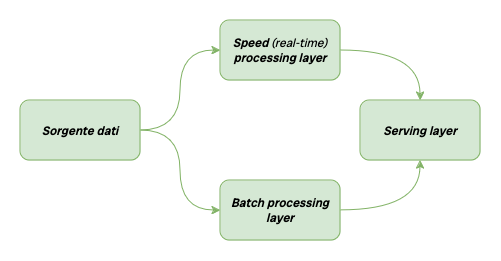
\includegraphics[width=0.6\textwidth]{./specifica_tecnica/architettura_lambda.png}
	\captionof{figure}{Architettura \textit{lambda}}
\end{center}

\subsubsubsection{Vantaggi e svantaggi}
L'architettura \textit{lambda} offre diversi vantaggi, tra cui la \textbf{scalabilità orizzontale}, la \textbf{tolleranza ai guasti} e la \textbf{flessibilità}. Tuttavia, la presenza
di due \textit{layer} di elaborazione separati può portare a problemi di coerenza dei dati, duplicazione della logica di aggregazione e complessità aggiuntiva nella gestione del sistema.
Inoltre, rispetto all'architettura \textit{kappa}, l'architettura \textit{lambda} può avere una latenza più elevata.

\subsubsubsection{Casi d'uso}
L'architettura \textit{lambda} è particolarmente adatta per applicazioni che richiedono sia un'analisi sui dati in tempo reale che un'analisi storica.

\subsubsection{Architettura \textit{kappa}}
L'architettura \textit{kappa} è stata introdotta per semplificare l'architettura \textit{lambda}, eliminando la necessità di gestire due \textit{layer} di elaborazione separati per il \textit{batch processing} e il \textit{real-time processing}.
Essa si divide in tre componenti principali:
\begin{itemize}
	\item \textbf{sorgente di dati}: \href{https://7last.github.io/docs/pb/documentazione-interna/glossario\#responsabile}{responsabile\textsubscript{G}} dell'acquisizione dei dati grezzi da diverse sorgenti;
	\item \textbf{\textit{processing layer}}: \href{https://7last.github.io/docs/pb/documentazione-interna/glossario\#responsabile}{responsabile\textsubscript{G}} dell'elaborazione dei dati in tempo reale, senza la necessità di separare i dati in \textit{batch} e \textit{real-time};
	\item \textbf{\textit{serving layer}}: \href{https://7last.github.io/docs/pb/documentazione-interna/glossario\#responsabile}{responsabile\textsubscript{G}} della fornitura dei dati elaborati in modo veloce ed affidabile.
\end{itemize}

\begin{center}
	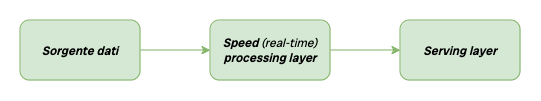
\includegraphics[width=0.6\textwidth]{./specifica_tecnica/architettura_kappa.png}
	\captionof{figure}{Architettura \textit{kappa}}
\end{center}

\subsubsubsection{Vantaggi e svantaggi}
L'architettura \textit{kappa} offre diversi vantaggi, tra cui la \textbf{semplicità}, la \textbf{riduzione dei costi} e la \textbf{bassa latenza}.
Tuttavia, può non essere adatta per applicazioni che richiedono un'analisi storica dei dati.

\subsubsubsection{Casi d'uso}
L'architettura \textit{kappa} è particolarmente adatta per gli scenari in cui sono critici i dati in tempo reale e l'analisi dei dati storici è meno importante. Inoltre, semplifica notevolmente il processo di sviluppo e manutenzione dei sistemi di elaborazione dei dati.

\subsection{Architettura scelta}
Nello scenario del \href{https://7last.github.io/docs/pb/documentazione-interna/glossario\#capitolato}{capitolato\textsubscript{G}} proposto da \textit{SyncLab S.r.L.}, è importante l'analisi in tempo reale, in quanto i dati provenienti dai sensori IoT devono fornire informazioni sempre aggiornate ed eventualmente
sollevare allarmi in caso di situazioni critiche. Inoltre, non è richiesta l'aggregazione storica di dati, dunque i vantaggi dell'architettura \textit{lambda} non risultano utili per i nostri fini.
Per soddisfare tali requisiti, è stata dunque scelta l'architettura \textit{kappa}.

\subsubsection{Componenti di sistema}
All'interno del sistema progettato sono dunque presenti le seguenti componenti:
\begin{itemize}
	\item \textbf{sorgenti di dati}: costituite dal simulatore di sensori, il quale genera i dati grezzi che in un contesto reale sarebbero provenienti dai sensori IoT;
	\item \textbf{\textit{streaming layer}}: gestisce il flusso di dati in tempo reale provenienti dai sensori. È composto da \href{https://7last.github.io/docs/pb/documentazione-interna/glossario\#redpanda}{\textit{Redpanda}\textsubscript{G}} e lo \href{https://7last.github.io/docs/pb/documentazione-interna/glossario\#schema-registry}{\textit{Schema Registry}\textsubscript{G}};
	\item \textbf{\textit{processing layer}}: elabora i dati in tempo reale per calcolare metriche e indici. È composto da \textit{Apache Flink};
	\item \textbf{\textit{storage layer}}: memorizza i dati elaborati per l'analisi e la visualizzazione. È composto da \href{https://7last.github.io/docs/pb/documentazione-interna/glossario\#clickhouse}{\textit{ClickHouse}\textsubscript{G}};
	\item \textbf{\textit{data visualization layer}}: fornisce un'interfaccia utente per visualizzare i dati elaborati. È composto da \href{https://7last.github.io/docs/pb/documentazione-interna/glossario\#grafana}{\textit{Grafana}\textsubscript{G}}.
\end{itemize}

\begin{center}
	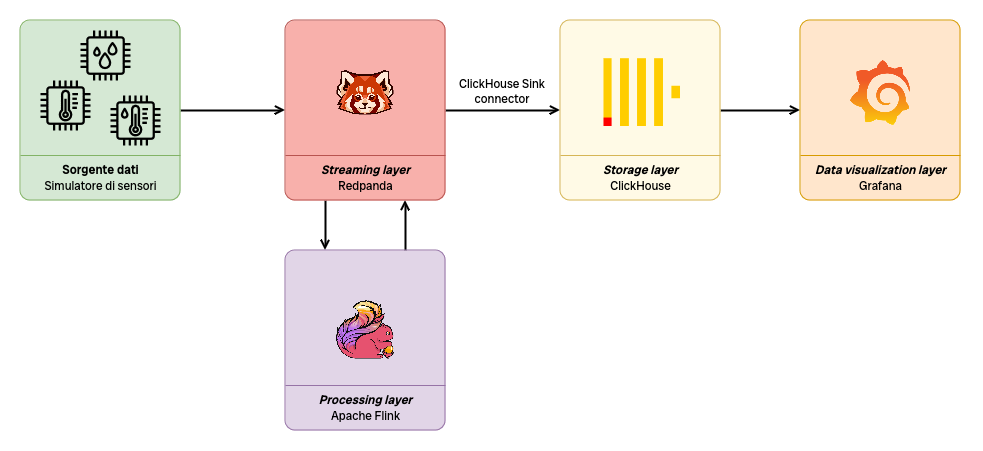
\includegraphics[width=0.9\textwidth]{./specifica_tecnica/architettura_sistema.png}
	\captionof{figure}{Componenti di sistema ad alto livello}
\end{center}

\subsubsection{Flusso di dati}
Per illustrare il flusso di dati all'interno del sistema, è stato realizzato il seguente diagramma, il quale mostra il percorso che i dati grezzi seguono dal simulatore fino alla visualizzazione tramite \href{https://7last.github.io/docs/pb/documentazione-interna/glossario\#grafana}{Grafana\textsubscript{G}}.
\begin{center}
	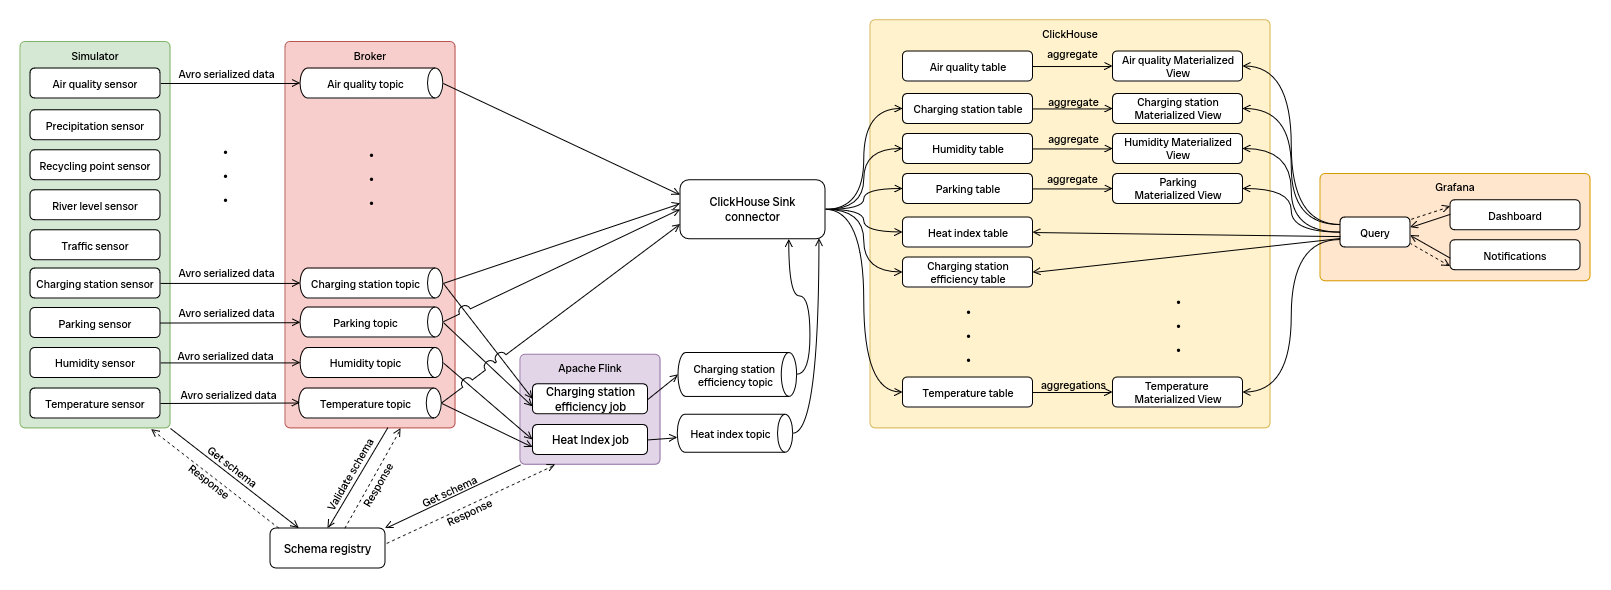
\includegraphics[width=1\textwidth]{./specifica_tecnica/data_flow.png}
	\captionof{figure}{Flusso di dati all'interno del sistema. I sensori di precipitazioni, isole ecologiche, livello dei fiumi e traffico sono stati omessi per chiarezza, ma il percorso di tali dati è analogo a quello dei sensori di qualità dell'aria.}
\end{center}
Il flusso seguito dai dati si può riassumere nei seguenti passaggi:
\begin{enumerate}
	\item \textbf{generazione dei dati}: ciascun simulatore emula il comportamento di un singolo \href{https://7last.github.io/docs/pb/documentazione-interna/glossario\#sensore}{sensore\textsubscript{G}} IoT, generando ad intervalli periodici o ad eventi (\textit{event-driven}) i dati grezzi relativi alla propria tipologia di dato.
	\item \textbf{serializzazione e produzione dei dati}: i dati grezzi generati nel punto precedente vengono serializzati utilizzando il formato Confluent Avro e inviati nel \href{https://7last.github.io/docs/pb/documentazione-interna/glossario\#topic}{\textit{topic}\textsubscript{G}} corrispondente al tipo di dato generato;
	\item \textbf{elaborazione dei dati}: i \href{https://7last.github.io/docs/pb/documentazione-interna/glossario\#topic}{\textit{topic}\textsubscript{G}} contenenti i dati grezzi di temperatura, umidità, occupazione dei parcheggi e colonnine di ricarica vengono consumati da Apache Flink.
	      Due \href{https://7last.github.io/docs/pb/documentazione-interna/glossario\#job}{\textit{job}\textsubscript{G}} distinti si occupano di calcolare la temperatura percepita e il grado di efficienza delle colonnine di ricarica. Una volta elaborati, i dati vengono inviati rispettivamente
	      nei \href{https://7last.github.io/docs/pb/documentazione-interna/glossario\#topic}{\textit{topic}\textsubscript{G}} \texttt{heat\_index} e \texttt{charging\_station\_efficiency};
	\item \textbf{memorizzazione dei dati}: attraverso il connettore \textit{sink} per \href{https://7last.github.io/docs/pb/documentazione-interna/glossario\#clickhouse}{ClickHouse\textsubscript{G}}, i dati pubblicati in tutti i \href{https://7last.github.io/docs/pb/documentazione-interna/glossario\#topic}{\textit{topic}\textsubscript{G}} vengono memorizzati nel database;
	\item \textbf{aggregazioni con \href{https://7last.github.io/docs/pb/documentazione-interna/glossario\#materialized-view}{\textit{materialized view}\textsubscript{G}}}: attraverso l'utilizzo di \href{https://7last.github.io/docs/pb/documentazione-interna/glossario\#materialized-view}{\textit{materialized view}\textsubscript{G}} in \href{https://7last.github.io/docs/pb/documentazione-interna/glossario\#clickhouse}{ClickHouse\textsubscript{G}}, vengono calcolate le statistiche relative ai dati memorizzati, come ad esempio la media oraria o giornaliera.
	      Tali aggregazioni sono più semplici rispetto a quelle effettuate da Flink, in quanto non richiedono elaborazioni complesse sui dati;
	\item \textbf{visualizzazione dei dati}: i dati memorizzati in \href{https://7last.github.io/docs/pb/documentazione-interna/glossario\#clickhouse}{ClickHouse\textsubscript{G}} vengono visualizzati tramite \href{https://7last.github.io/docs/pb/documentazione-interna/glossario\#grafana}{Grafana\textsubscript{G}}, che permette di creare \href{https://7last.github.io/docs/pb/documentazione-interna/glossario\#dashboard}{\textit{dashboard}\textsubscript{G}} personalizzate per monitorare i dati in tempo reale;
	\item \textbf{notifiche}: \href{https://7last.github.io/docs/pb/documentazione-interna/glossario\#grafana}{Grafana\textsubscript{G}} esegue periodicamente delle \textit{query} per verificare se sono state superate delle soglie predeterminate. In caso affermativo, vengono inviate notifiche tramite il canale Discord dedicato, in modo tale da poter avvisare l'autorità locale.
\end{enumerate}

\subsection{Architettura dei simulatori}
I simulatori vengono utilizzati per produrre dati grezzi che sostituiscono le rilevazioni effettuate dai sensori IoT in un contesto reale.
Per tale motivo, questa parte del sistema non è ufficialmente parte del prodotto finale, ma è stata sviluppata per scopi di \textit{test}
e dimostrativi nell'ambito del progetto didattico; ai fini di quest'ultimo, il gruppo ha deciso di dedicare alcune risorse per la progettazione.\\
Nei paragrafi successivi verranno descritti i moduli che compongono i simulatori, le classi e metodi principali e i \href{https://7last.github.io/docs/pb/documentazione-interna/glossario\#design-pattern}{\textit{design pattern}\textsubscript{G}} utilizzati.\\
Sono stati implementati simulatori per i seguenti tipi dato:
\begin{itemize}
	\item qualità dell'aria;
	\item precipitazioni;
	\item isole ecologiche;
	\item livello dei fiumi;
	\item traffico;
	\item colonnine di ricarica;
	\item parcheggi;
	\item temperatura;
	\item umidità.
\end{itemize}

\subsubsection{Modulo \texttt{models}}
Questo modulo contiene le classi che rappresentano i dati grezzi generati dai sensori (sottomodulo \texttt{raw\_data}) e la configurazione dei sensori stessi (sottomodulo \texttt{config}) letta
dal file di configurazione \texttt{sensors.\href{https://7last.github.io/docs/pb/documentazione-interna/glossario\#tom's-obvious-minimal-language}{toml\textsubscript{G}}} e dalle variabili d'ambiente.\\
Ciascun tipo di dato grezzo è rappresentato da una classe che estende \texttt{RawData} (astratta).\\
La classe \texttt{SensorConfig} riceve nel costruttore la configurazione sotto forma di dizionario, effettua \textit{parsing}, validazione,
popola con valori di \textit{default} i campi mancanti (nel caso lo prevedano) ed inizializza i propri attributi, corrispondenti ai campi del file di configurazione.\\
Allo stesso modo, \texttt{EnvConfig} legge le variabili d'ambiente ed espone il metodo \\\texttt{bootstrap\_server()} che combina \textit{host} e \textit{port} per formare l'indirizzo del \href{https://7last.github.io/docs/pb/documentazione-interna/glossario\#broker}{\textit{broker}\textsubscript{G}} Kafka.\\
\begin{center}
	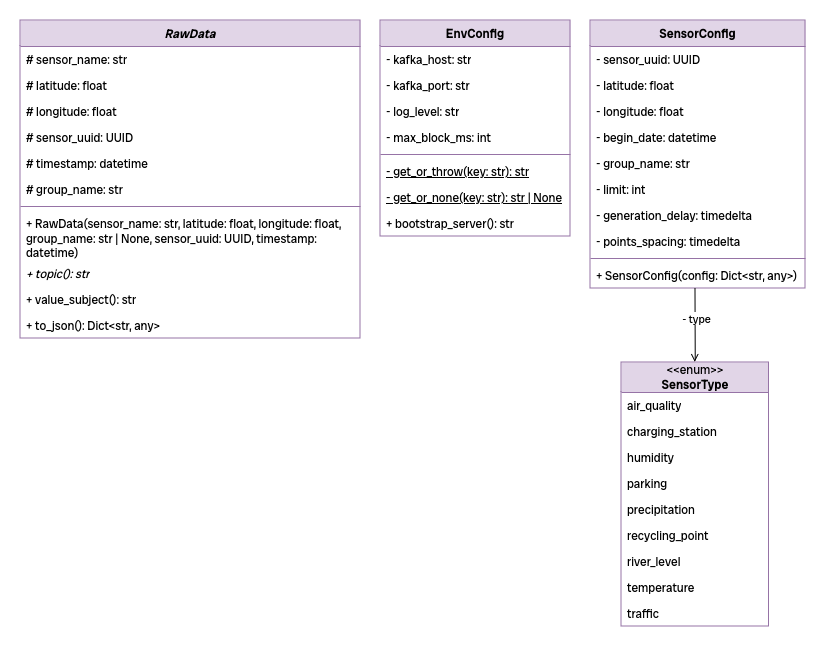
\includegraphics[width=0.87\textwidth]{./specifica_tecnica/models.png}
	\captionof{figure}{Diagramma delle classi del modulo \texttt{models}. Per ragioni di spazio, le implementazioni di \texttt{RawData} sono illustrate nel diagramma successivo}
\end{center}

\subsubsubsection{Classi, interfacce metodi e attributi}
\begin{itemize}
	\item \textbf{Classe astratta \texttt{RawData}}:
	      \begin{itemize}
		      \item \textbf{Attributi}
		            \begin{itemize}
			            \item \texttt{sensor\_uuid} string [protected]: identificativo univoco del \href{https://7last.github.io/docs/pb/documentazione-interna/glossario\#sensore}{sensore\textsubscript{G}};
			            \item \texttt{latitude} float [protected]: latitudine del \href{https://7last.github.io/docs/pb/documentazione-interna/glossario\#sensore}{sensore\textsubscript{G}};
			            \item \texttt{longitude} float [protected]: longitudine del \href{https://7last.github.io/docs/pb/documentazione-interna/glossario\#sensore}{sensore\textsubscript{G}};
			            \item \texttt{sensor\_name} string [protected]: nome del \href{https://7last.github.io/docs/pb/documentazione-interna/glossario\#sensore}{sensore\textsubscript{G}};
			            \item \texttt{group\_name} string [protected]: nome del gruppo di sensori a cui appartiene.
		            \end{itemize}
		      \item \textbf{Metodi}
		            \begin{itemize}
			            \item \href{https://7last.github.io/docs/pb/documentazione-interna/glossario\#topic}{\texttt{topic}\textsubscript{G}}\texttt{()} string [public,abstract]: restituisce il nome del \href{https://7last.github.io/docs/pb/documentazione-interna/glossario\#topic}{\textit{topic}\textsubscript{G}} in cui i dati grezzi vanno pubblicati;
			            \item \texttt{value\_subject()} string [public]: restituisce il nome del campo value del record.
		            \end{itemize}
	      \end{itemize}
	\item \textbf{Classe EnvConfig}:
	      \begin{itemize}
		      \item \textbf{Attributi}
		            \begin{itemize}
			            \item \texttt{kafka\_host} string [private]: \textit{host} del \href{https://7last.github.io/docs/pb/documentazione-interna/glossario\#broker}{\textit{broker}\textsubscript{G}} Kafka;
			            \item \texttt{kafka\_port} string [private]: porta del \href{https://7last.github.io/docs/pb/documentazione-interna/glossario\#broker}{\textit{broker}\textsubscript{G}} Kafka;
			            \item \texttt{log\_level} string [private]: livello di \textit{logging} da utilizzare;
			            \item \texttt{max\_block\_ms} int [private]: tempo massimo di blocco per la produzione di messaggi.
		            \end{itemize}
		      \item \textbf{Metodi}
		            \begin{itemize}
			            \item \texttt{get\_or\_throw(key: string)} string [private,static]: restituisce il valore della variable d'ambiente associato alla chiave \texttt{key} se presente, altrimenti lancia un'eccezione;
			            \item \texttt{get\_or\_none(key: string)} string [private,static]: restituisce il valore della variable d'ambiente associato alla chiave \texttt{key} se presente, altrimenti \texttt{None};
			            \item \texttt{bootstrap\_server()} string [public]: restituisce l'indirizzo del \href{https://7last.github.io/docs/pb/documentazione-interna/glossario\#broker}{\textit{broker}\textsubscript{G}} Kafka.
		            \end{itemize}
	      \end{itemize}
	\item \textbf{Classe SensorConfig}:
	      \begin{itemize}
		      \item \textbf{Attributi}
		            \begin{itemize}
			            \item \texttt{sensor\_uuid} string [private]: identificativo univoco del \href{https://7last.github.io/docs/pb/documentazione-interna/glossario\#sensore}{sensore\textsubscript{G}};
			            \item \texttt{limit} int [private]: limite massimo di misurazioni da effettuare;
			            \item \texttt{begin\_date} datetime [private]: data e ora di inizio delle misurazioni;
			            \item \texttt{latitude} float [private]: latitudine del \href{https://7last.github.io/docs/pb/documentazione-interna/glossario\#sensore}{sensore\textsubscript{G}};
			            \item \texttt{longitude} float [private]: longitudine del \href{https://7last.github.io/docs/pb/documentazione-interna/glossario\#sensore}{sensore\textsubscript{G}};
			            \item \texttt{group\_name} string [private]: nome del gruppo di sensori a cui appartiene;
			            \item \texttt{type} SensorType [private]: tipo di \href{https://7last.github.io/docs/pb/documentazione-interna/glossario\#sensore}{sensore\textsubscript{G}};
			            \item \texttt{points\_spacing} timedelta [private]: intervallo temporale tra due misurazioni;
			            \item \texttt{generation\_delay} timedelta [private]: ritardo tra la generazione di due misurazioni adiacenti.
		            \end{itemize}
	      \end{itemize}
	\item \href{https://7last.github.io/docs/pb/documentazione-interna/glossario\#enumerazione}{\textbf{Enum}\textsubscript{G}}\textbf{ SensorType}:
	      \begin{itemize}
		      \item \textbf{Valori}
		            \begin{itemize}
			            \item \texttt{AIR\_QUALITY}
			            \item \texttt{PARKING}
			            \item \texttt{RECYCLING\_POINT}
			            \item \texttt{TEMPERATURE}
			            \item \texttt{TRAFFIC}
			            \item \texttt{CHARGING\_STATION}
			            \item \texttt{PRECIPITATION}
			            \item \texttt{RIVER\_LEVEL}
			            \item \texttt{HUMIDITY}
		            \end{itemize}
		      \item \textbf{Metodi}
		            \begin{itemize}
			            \item \texttt{from\_str(value: string)} SensorType [public,static]: restituisce il valore dell'\href{https://7last.github.io/docs/pb/documentazione-interna/glossario\#enumerazione}{enum\textsubscript{G}} corrispondente alla stringa \texttt{value}.
		            \end{itemize}
	      \end{itemize}
	\item \textbf{Classe AirQualityRawData}
	      \begin{itemize}
		      \item \textbf{Metodi}:
		            \begin{itemize}
			            \item \href{https://7last.github.io/docs/pb/documentazione-interna/glossario\#topic}{\texttt{topic}\textsubscript{G}}\texttt{()} str [public]: restituisce il nome del \href{https://7last.github.io/docs/pb/documentazione-interna/glossario\#topic}{\textit{topic}\textsubscript{G}} in cui i dati grezzi vanno pubblicati.
		            \end{itemize}
	      \end{itemize}
	\item \textbf{Classe ChargingStationRawData}
	      \begin{itemize}
		      \item \textbf{Metodi}:
		            \begin{itemize}
			            \item \href{https://7last.github.io/docs/pb/documentazione-interna/glossario\#topic}{\texttt{topic}\textsubscript{G}}\texttt{()} str [public]: restituisce il nome del \href{https://7last.github.io/docs/pb/documentazione-interna/glossario\#topic}{\textit{topic}\textsubscript{G}} in cui i dati grezzi vanno pubblicati.
		            \end{itemize}
	      \end{itemize}
	\item \textbf{Classe HumidityRawData}
	      \begin{itemize}
		      \item \textbf{Metodi}:
		            \begin{itemize}
			            \item \href{https://7last.github.io/docs/pb/documentazione-interna/glossario\#topic}{\texttt{topic}\textsubscript{G}}\texttt{()} str [public]: restituisce il nome del \href{https://7last.github.io/docs/pb/documentazione-interna/glossario\#topic}{\textit{topic}\textsubscript{G}} in cui i dati grezzi vanno pubblicati.
		            \end{itemize}
	      \end{itemize}
	\item \textbf{Classe ParkingRawData}
	      \begin{itemize}
		      \item \textbf{Metodi}:
		            \begin{itemize}
			            \item \href{https://7last.github.io/docs/pb/documentazione-interna/glossario\#topic}{\texttt{topic}\textsubscript{G}}\texttt{()} str [public]: restituisce il nome del \href{https://7last.github.io/docs/pb/documentazione-interna/glossario\#topic}{\textit{topic}\textsubscript{G}} in cui i dati grezzi vanno pubblicati.
		            \end{itemize}
	      \end{itemize}
	\item \textbf{Classe PrecipitationRawData}
	      \begin{itemize}
		      \item \textbf{Metodi}:
		            \begin{itemize}
			            \item \href{https://7last.github.io/docs/pb/documentazione-interna/glossario\#topic}{\texttt{topic}\textsubscript{G}}\texttt{()} str [public]: restituisce il nome del \href{https://7last.github.io/docs/pb/documentazione-interna/glossario\#topic}{\textit{topic}\textsubscript{G}} in cui i dati grezzi vanno pubblicati.
		            \end{itemize}
	      \end{itemize}
	\item \textbf{Classe RecyclingPointRawData}
	      \begin{itemize}
		      \item \textbf{Metodi}:
		            \begin{itemize}
			            \item \href{https://7last.github.io/docs/pb/documentazione-interna/glossario\#topic}{\texttt{topic}\textsubscript{G}}\texttt{()} str [public]: restituisce il nome del \href{https://7last.github.io/docs/pb/documentazione-interna/glossario\#topic}{\textit{topic}\textsubscript{G}} in cui i dati grezzi vanno pubblicati.
		            \end{itemize}
	      \end{itemize}
	\item \textbf{Classe RiverLevelRawData}
	      \begin{itemize}
		      \item \textbf{Metodi}:
		            \begin{itemize}
			            \item \href{https://7last.github.io/docs/pb/documentazione-interna/glossario\#topic}{\texttt{topic}\textsubscript{G}}\texttt{()} str [public]: restituisce il nome del \href{https://7last.github.io/docs/pb/documentazione-interna/glossario\#topic}{\textit{topic}\textsubscript{G}} in cui i dati grezzi vanno pubblicati.
		            \end{itemize}
	      \end{itemize}
	\item \textbf{Classe TemperatureRawData}
	      \begin{itemize}
		      \item \textbf{Metodi}:
		            \begin{itemize}
			            \item \href{https://7last.github.io/docs/pb/documentazione-interna/glossario\#topic}{\texttt{topic}\textsubscript{G}}\texttt{()} str [public]: restituisce il nome del \href{https://7last.github.io/docs/pb/documentazione-interna/glossario\#topic}{\textit{topic}\textsubscript{G}} in cui i dati grezzi vanno pubblicati.
		            \end{itemize}
	      \end{itemize}
	\item \textbf{Classe TrafficRawData}
	      \begin{itemize}
		      \item \textbf{Metodi}:
		            \begin{itemize}
			            \item \href{https://7last.github.io/docs/pb/documentazione-interna/glossario\#topic}{\texttt{topic}\textsubscript{G}}\texttt{()} str [public]: restituisce il nome del \href{https://7last.github.io/docs/pb/documentazione-interna/glossario\#topic}{\textit{topic}\textsubscript{G}} in cui i dati grezzi vanno pubblicati.
		            \end{itemize}
	      \end{itemize}
\end{itemize}

\subsubsection{Modulo \texttt{simulators}}
Il modulo \texttt{simulators} contiene la logica per la generazione dei dati grezzi e l'orchestrazione dei simulatori.\\
L'\textit{entrypoint} di tutto il sistema è la classe \texttt{SimulatorExecutor}, che riceve la configurazione dei sensori
ed utilizzando il \texttt{SimulatorFactory} crea un \texttt{SimulatorThread} per ogni \href{https://7last.github.io/docs/pb/documentazione-interna/glossario\#sensore}{sensore\textsubscript{G}}.
Quest'ultimo, a partire da una \texttt{SimulatorStrategy} ed una \texttt{ProducerStrategy}, genera i dati grezzi e li invia al \texttt{Producer}.\\
La classe \texttt{SimulatorThread} utilizza un \texttt{threading.Event}, che contiene un \textit{flag} booleano.
Quest'ultimo può essere impostato a \texttt{True} per far partire il \textit{thread}; il metodo \texttt{wait()} permette di mettere in attesa il \textit{thread} fino a quando il \textit{flag} è
impostato a \texttt{True}, per un periodo di tempo massimo espresso dal parametro \texttt{timeout}.\\ Tale metodo è utilizzato per attendere un determinato periodo di tempo tra la generazione di due misurazioni.\\

\begin{center}
	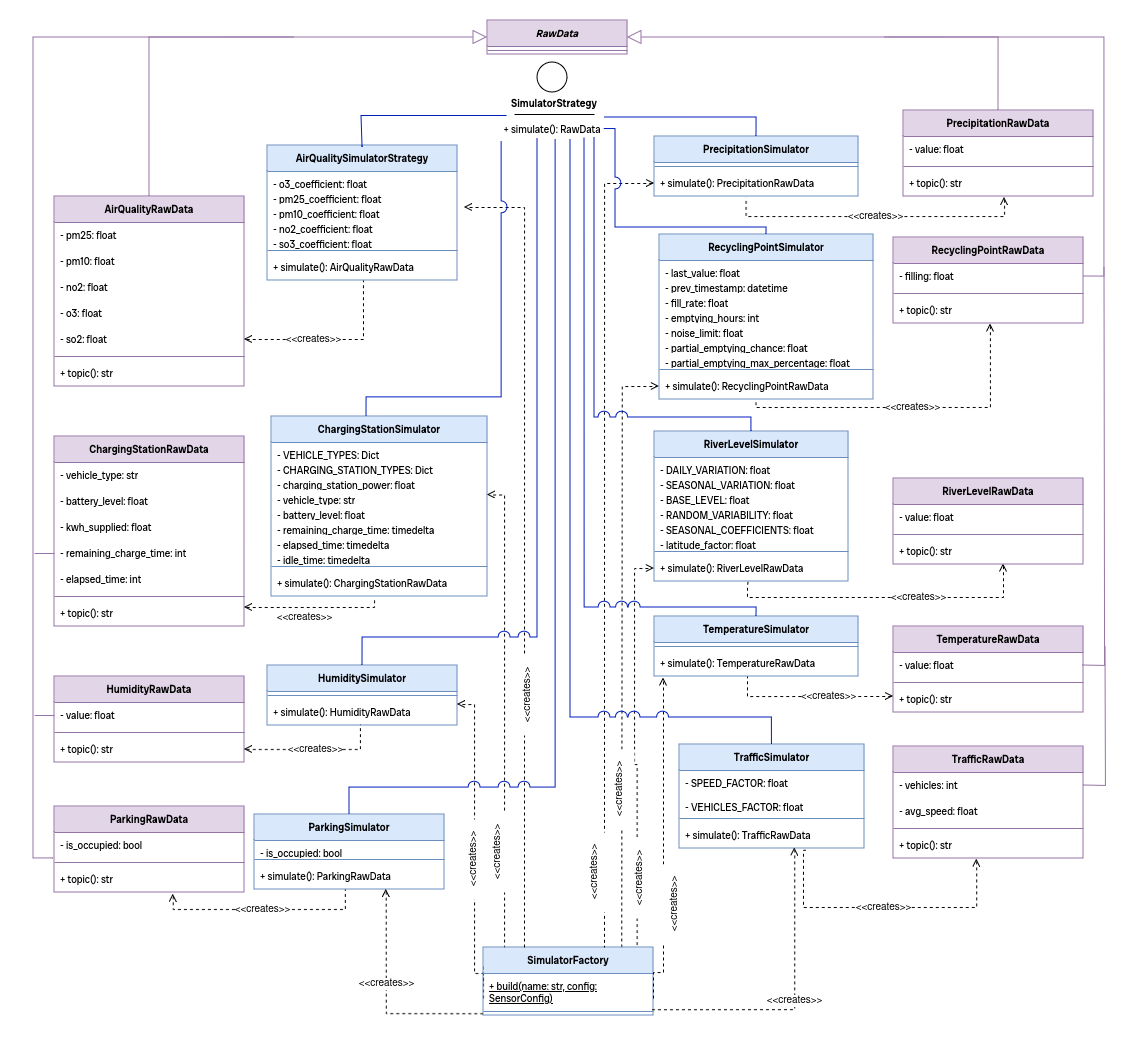
\includegraphics[width=1\textwidth]{./specifica_tecnica/simulators.png}
	\captionof{figure}{Diagramma delle classi modulo \texttt{simulators} e \texttt{models}.}
\end{center}

\subsubsubsection{\textit{Design Pattern}}
\subsubsubsubsection{\textit{Strategy}}
All'interno del modulo \texttt{simulators} è stato utilizzato il \href{https://7last.github.io/docs/pb/documentazione-interna/glossario\#design-pattern}{\textit{design pattern}\textsubscript{G}} \textit{Strategy} per permettere la generazione di dati grezzi di diversi tipi.
Ciascuna tipologia simulatore implementa l'interfaccia \texttt{SimulatorStrategy} che definisce il metodo \texttt{simulate()}. In questo modo, la classe \texttt{SimulatorThread}
può eseguire il simulatore senza conoscere il tipo di dato generato, rendendo inoltre semplice l'aggiunta di nuovi tipi di dati grezzi senza dover modificare il codice esistente.

\subsubsubsubsection{\textit{Factory}}
La classe \texttt{SimulatorFactory} implementa il \href{https://7last.github.io/docs/pb/documentazione-interna/glossario\#design-pattern}{\textit{design pattern}\textsubscript{G}} \textit{Factory}, fornendo un metodo che si occupa della creazione dei simulatori
a partire da un valore dell'\href{https://7last.github.io/docs/pb/documentazione-interna/glossario\#enumerazione}{enum\textsubscript{G}} \texttt{SensorType}.


\subsubsubsection{Classi, interfacce metodi e attributi}
\begin{itemize}
	\item \textbf{Classe SimulatorExecutor}
	      \begin{itemize}
		      \item \textbf{Attributi}:
		            \begin{itemize}
			            \item \texttt{simulator\_threads} List[SimulatorThread] [private]: lista dei simulatori da eseguire;
			            \item \texttt{stop\_event}: threading.Event [private]: evento utilizzato per tenere attivo il \textit{thread} principale dopo aver lanciato i \textit{thread} dei simulatori.
		            \end{itemize}
		      \item \textbf{Metodi}:
		            \begin{itemize}
			            \item \texttt{stop\_all()} None [public]:
			            \item \texttt{run()} None [public]:
		            \end{itemize}
	      \end{itemize}
	\item \textbf{Classe SimulatorFactory}
	      \begin{itemize}
		      \item \textbf{Metodi}:
		            \begin{itemize}
			            \item \texttt{build(name: str, config: SensorConfig)} SimulatorStrategy [public, static]: restituisce un'istanza del simulatore \\ corrispondente al nome \texttt{name}.
		            \end{itemize}
	      \end{itemize}
	\item \textbf{Interfaccia SimulatorStrategy}
	      \begin{itemize}
		      \item \textbf{Attributi}:
		            \begin{itemize}
			            \item \texttt{generation\_delay} timedelta [protected]: ritardo tra la generazione di due misurazioni adiacenti.
			            \item \texttt{group\_name} str [protected]: nome del gruppo di sensori a cui appartiene il \href{https://7last.github.io/docs/pb/documentazione-interna/glossario\#sensore}{sensore\textsubscript{G}};
			            \item \texttt{latitude} float [protected]: latitudine del \href{https://7last.github.io/docs/pb/documentazione-interna/glossario\#sensore}{sensore\textsubscript{G}};
			            \item \texttt{limit} int [protected]: limite massimo di misurazioni da produrre;
			            \item \texttt{longitude} float [protected]: longitudine del \href{https://7last.github.io/docs/pb/documentazione-interna/glossario\#sensore}{sensore\textsubscript{G}};
			            \item \texttt{points\_spacing} timedelta [protected]: intervallo temporale tra due misurazioni;
			            \item \texttt{sensor\_name} str [protected]: nome del \href{https://7last.github.io/docs/pb/documentazione-interna/glossario\#sensore}{sensore\textsubscript{G}} per cui il simulatore genera dati;
			            \item \texttt{sensor\_uuid} str [protected]: identificativo univoco del \href{https://7last.github.io/docs/pb/documentazione-interna/glossario\#sensore}{sensore\textsubscript{G}} per cui il simulatore genera dati;
			            \item \texttt{timestamp} datetime [protected]: data e ora dell'ultima misurazione;
		            \end{itemize}
		      \item \textbf{Metodi}:
		            \begin{itemize}
			            \item \texttt{simulate} RawData [public]: metodo che simula la generazione di dati grezzi;
		            \end{itemize}
	      \end{itemize}
	\item \textbf{Classe SimulatorThread}
	      \begin{itemize}
		      \item \textbf{Attributi}:
		            \begin{itemize}
			            \item \texttt{simulator} SimulatorStrategy [private]: simulatore da eseguire;
			            \item \texttt{event} threading.Event [private]: evento utilizzato per fermare, far partire o lasciare in attesa il \textit{thread} del simulatore.
		            \end{itemize}
		      \item \textbf{Metodi}:
		            \begin{itemize}
			            \item \texttt{run()} None [public]: esegue il simulatore;
			            \item \texttt{is\_running()} bool [public]: restituisce \texttt{True} se il \textit{thread} è in esecuzione, \texttt{False} altrimenti;
			            \item \texttt{stop()} None [public]: ferma il \textit{thread} del simulatore.
		            \end{itemize}
	      \end{itemize}
	\item \textbf{Classe AirQualitySimulatorStrategy}
	      \begin{itemize}
		      \item \textbf{Attributi}:
		            \begin{itemize}
			            \item \texttt{o3\_coefficient} float [private]: coefficiente randomico utilizzato per generare il valore di \texttt{o3};
			            \item \texttt{pm25\_coefficient} float [private]: coefficiente randomico utilizzato per generare il valore di \texttt{pm25};
			            \item \texttt{pm10\_coefficient} float [private]: coefficiente randomico utilizzato per generare il valore di \texttt{pm10};
			            \item \texttt{no2\_coefficient} float [private]: coefficiente randomico utilizzato per generare il valore di \texttt{no2};
			            \item \texttt{so2\_coefficient} float [private]: coefficiente randomico utilizzato per generare il valore di \texttt{so2};
		            \end{itemize}
		      \item \textbf{Metodi}:
		            \begin{itemize}
			            \item \texttt{simulate()} AirQualityRawData [public]: genera un dato di tipo AirQualityRawData;
		            \end{itemize}
	      \end{itemize}
	\item \textbf{Classe ChargingStationSimulatorStrategy}
	      \begin{itemize}
		      \item \textbf{Attributi}:
		            \begin{itemize}
			            \item \texttt{VEHICLE\_TYPES}: Dict[str, Dict[str, float]] [private]: dizionario contenente i tipi di veicoli supportati e la capacità minima e massima della batteria;
			            \item \texttt{CHARGING\_STATION\_TYPES} Dict[str, Dict[str, float]] [private]: dizionario contenente i tipi di colonnine di ricarica supportati e la potenza minima e massima;
			            \item \texttt{charging\_station\_power} float [private]: potenza della colonnina di ricarica;
			            \item \texttt{vehicle\_type} str [private]: tipo di veicolo supportato dalla colonnina di ricarica;
			            \item \texttt{battery\_level} float [private]: livello di carica della batteria;
			            \item \texttt{remaining\_charge\_time} timedelta [private]: tempo rimanente per completare la ricarica;
			            \item \texttt{elapsed\_time} timedelta [private]: tempo trascorso dall'inizio della ricarica;
			            \item \texttt{idle\_time} timedelta [private]: tempo in cui la colonnina di ricarica è inattiva;
		            \end{itemize}
		      \item \textbf{Metodi}:
		            \begin{itemize}
			            \item \texttt{simulate()} ChargingStationRawData [public]: genera un dato di
			                  tipo \\ChargingStationRawData;
		            \end{itemize}
	      \end{itemize}
	\item \textbf{Classe HumiditySimulatorStrategy}
	      \begin{itemize}
		      \item \textbf{Metodi}:
		            \begin{itemize}
			            \item \texttt{simulate()} HumidityRawData [public]: genera un dato di tipo HumidityRawData;
		            \end{itemize}
	      \end{itemize}
	\item \textbf{Classe ParkingSimulatorStrategy}
	      \begin{itemize}
		      \item \textbf{Attributi}:
		            \begin{itemize}
			            \item \texttt{is\_occupied} bool [private]: indica se il parcheggio è occupato;
		            \end{itemize}
		      \item \textbf{Metodi}:
		            \begin{itemize}
			            \item \texttt{simulate()} ParkingRawData [public]: genera un dato di tipo ParkingRawData;
		            \end{itemize}
	      \end{itemize}
	\item \textbf{Classe PrecipitationSimulatorStrategy}
	      \begin{itemize}
		      \item \textbf{Metodi}:
		            \begin{itemize}
			            \item \texttt{simulate()} PrecipitationRawData [public]: genera un dato di tipo\\ PrecipitationRawData;
		            \end{itemize}
	      \end{itemize}
	\item \textbf{Classe RecyclingPointSimulatorStrategy}
	      \begin{itemize}
		      \item \textbf{Attributi}:
		            \begin{itemize}
			            \item \texttt{last\_value} float [private]: ultimo valore generato;
			            \item \texttt{prev\_timestamp} datetime [private]: data e ora dell'ultima misurazione;
			            \item \texttt{fill\_rate} float [private]: tasso di riempimento del contenitore;
			            \item \texttt{emptying\_hours} int [private]: ore necessarie per svuotare il contenitore;
			            \item \texttt{noise\_limit} float [private]: quantità massima di rumore da aggiungere al valore generato;
			            \item \texttt{partial\_emptying\_chance} float [private]: probabilità di svuotamento parziale;
			            \item \texttt{partial\_emptying\_max\_percentage} float [private]: percentuale massima di svuotamento parziale;
		            \end{itemize}
		      \item \textbf{Metodi}:
		            \begin{itemize}
			            \item \texttt{simulate()} RecyclingPointRawData [public]: genera un dato di tipo\\ RecyclingPointRawData;
		            \end{itemize}
	      \end{itemize}
	\item \textbf{Classe RiverLevelSimulatorStrategy}
	      \begin{itemize}
		      \item \textbf{Attributi}:
		            \begin{itemize}
			            \item \texttt{DAILY\_VARIATION} float [private]: variazione giornaliera massima del livello del fiume;
			            \item \texttt{SEASONAL\_VARIATION} float [private]: variazione stagionale massima del livello del fiume;
			            \item \texttt{BASE\_LEVEL} float [private]: livello base del fiume;
			            \item \texttt{RANDOM\_VARIABILITY} float [private]: massima variazione casuale del livello del fiume;
			            \item \texttt{SEASONAL\_COEFFICIENTS} Dict[int, float] [private]: coefficienti stagionali per la variazione del livello del fiume;
			            \item \texttt{latitude\_factor} float [private]: fattore moltiplicativo per la latitudine;
		            \end{itemize}
		      \item \textbf{Metodi}:
		            \begin{itemize}
			            \item \texttt{simulate()} RiverLevelRawData [public]: genera un dato di tipo RiverLevelRawData;
		            \end{itemize}
	      \end{itemize}
	\item \textbf{Classe TemperatureSimulatorStrategy}
	      \begin{itemize}
		      \item \textbf{Metodi}:
		            \begin{itemize}
			            \item \texttt{simulate()} TemperatureRawData [public]: genera un dato di tipo\\ TemperatureRawData;
		            \end{itemize}
	      \end{itemize}
	\item \textbf{Classe TrafficSimulatorStrategy}
	      \begin{itemize}
		      \item \textbf{Attributi}:
		            \begin{itemize}
			            \item \texttt{SPEED\_FACTOR} float [private]: fattore moltiplicativo per la velocità;
			            \item \texttt{VEHICLES\_FACTOR} [private]: fattore moltiplicativo per il numero di veicoli;
		            \end{itemize}
		      \item \textbf{Metodi}:
		            \begin{itemize}
			            \item \texttt{simulate()} TrafficRawData [public]: genera un dato di tipo TrafficRawData;
		            \end{itemize}
	      \end{itemize}

\end{itemize}

\subsubsection{Modulo \texttt{producers}}
Il modulo \texttt{producers} contiene le classi che si occupano della produzione dei dati grezzi.
\subsubsubsection{Design Pattern}
\subsubsubsubsection{\textit{Strategy}}
Analogamente a quanto effettuato nel modulo \texttt{simulators}, anche in questo caso è stato utilizzato il \href{https://7last.github.io/docs/pb/documentazione-interna/glossario\#design-pattern}{\textit{design pattern}\textsubscript{G}} \textit{Strategy} per permettere la produzione di dati grezzi di diversi tipi.
Sono stati implementati due produttori: \texttt{KafkaProducerAdapter} e \texttt{StdOutProducer}, rispettivamente per la produzione di dati su Kafka e su \textit{standard output}.

\subsubsubsubsection{\textit{Object Adapter}}
Al fine di adattare la classe \texttt{KafkaProducer}, contenuta nella libreria \texttt{kafka}, abbiamo utilizzato il \href{https://7last.github.io/docs/pb/documentazione-interna/glossario\#design-pattern}{\textit{design pattern}\textsubscript{G}} \textit{Adapter}, nella sua variante
\textit{Object Adapter}. Esso consente di rendere compatibile con l'interfaccia \texttt{ProducerStrategy} la classe \texttt{KafkaProducer}, la quale potrebbe subire
cambiamenti da noi non controllabili. In tale eventualità, il \textit{pattern} \textit{Adapter} consente di poter continuare ad utilizzare tale classe senza dover modificare altre parti del sistema.

\subsubsubsection{Classi, interfacce metodi e attributi}
\begin{itemize}
	\item \textbf{Interfaccia ProducerStrategy}
	      \begin{itemize}
		      \item \textbf{Attributi}:
		            \begin{itemize}
			            \item \texttt{serialization\_strategy} SerializationStrategy [protected]: strategia di serializzazione dei dati grezzi.
		            \end{itemize}
		      \item \textbf{Metodi}:
		            \begin{itemize}
			            \item \texttt{produce(data: RawData)} bool [public]: metodo che produce i dati grezzi in base alla strategia utilizzata, ritornando \texttt{True} in caso di successo, \texttt{False} altrimenti.
		            \end{itemize}
	      \end{itemize}
	\item \textbf{Classe KafkaProducerAdapter}
	      \begin{itemize}
		      \item \textbf{Attributi}:
		            \begin{itemize}
			            \item \texttt{serialization\_strategy} SerializationStrategy [protected]: strategia di serializzazione dei dati grezzi.
			            \item \texttt{adaptee} KafkaProducer [private]: produttore di dati su Kafka.
		            \end{itemize}
		      \item \textbf{Metodi}:
		            \begin{itemize}
			            \item \texttt{produce(data: RawData)} bool [public]: produce i dati grezzi su Kafka, ritornando \texttt{True} in caso di successo, \texttt{False} altrimenti.
		            \end{itemize}
		      \item \textbf{Note}:
		            \begin{itemize}
			            \item la classe \texttt{KafkaProducerAdapter} si appoggia alla libreria \texttt{kafka} per interagire con il \href{https://7last.github.io/docs/pb/documentazione-interna/glossario\#broker}{\textit{broker}\textsubscript{G}}, realizzando
			                  il \textit{pattern} \textit{Adapter} per adattare la classe \texttt{KafkaProducer} all'interfaccia \texttt{ProducerStrategy}.
		            \end{itemize}
	      \end{itemize}
	\item \textbf{Classe StdOutProducer}
	      \begin{itemize}
		      \item \textbf{Attributi}:
		            \begin{itemize}
			            \item \texttt{serialization\_strategy} SerializationStrategy [protected]: strategia di serializzazione dei dati grezzi.
		            \end{itemize}
		      \item \textbf{Metodi}:
		            \begin{itemize}
			            \item \texttt{produce(data: RawData)} bool [public]: produce i dati grezzi su \textit{standard output}.
		            \end{itemize}
	      \end{itemize}
\end{itemize}

\subsubsection{Modulo \texttt{serializers}}
Il modulo \texttt{serializers} contiene le classi che si occupano della serializzazione dei dati grezzi. Questi vengono serializzati in due formati: \href{https://7last.github.io/docs/pb/documentazione-interna/glossario\#javascript-object-notation}{JSON\textsubscript{G}} e Confluent Avro.
La serializzazione in \href{https://7last.github.io/docs/pb/documentazione-interna/glossario\#javascript-object-notation}{JSON\textsubscript{G}} viene principalmente utilizzata per il \textit{debugging} e la visualizzazione dei dati grezzi su \textit{standard output}, mentre la serializzazione in Avro
per l'effettiva produzione dei dati su Kafka.

\subsubsubsection{\textit{Design Pattern}}
\subsubsubsubsection{\textit{Strategy}}
Abbiamo deciso di utilizzare il \href{https://7last.github.io/docs/pb/documentazione-interna/glossario\#design-pattern}{\textit{design pattern}\textsubscript{G}} \textit{Strategy} per serializzare le istanze di \texttt{RawData} in \textit{byte} utilizzando diverse codifiche, senza dover modificare il codice che le utilizza;
per tale motivo sono state implementate le classi \\\texttt{JsonSerializationStrategy} e \texttt{AvroSerializationStrategy}.
\texttt{DictSerializable} è un'interfaccia che definisce il metodo \texttt{to\_dict()}, il quale restituisce un dizionario \href{https://7last.github.io/docs/pb/documentazione-interna/glossario\#python}{Python\textsubscript{G}}.
L'interfaccia \texttt{SerializationStrategy} definisce il metodo \texttt{serialize(data: DictSerializable)}, che prende in input un \texttt{DictSerializable} restituisce i \textit{byte} corrispondenti.
\\\texttt{AvroSerializationStrategy} si appoggia sulla libreria \texttt{confluent\_avro} per interagire con lo \href{https://7last.github.io/docs/pb/documentazione-interna/glossario\#schema-registry}{\textit{schema registry}\textsubscript{G}} e costruire un oggetto di tipo
\texttt{AvroValueSerde}, necessario per la serializzazione a partire da uno schema Avro e un dizionario.

\subsubsubsubsection{\textit{Object Adapter}}
Entrambe le classi \texttt{JsonSerializationStrategy} e \texttt{AvroSerializationStrategy} necessitano di convertire un oggetto di tipo \texttt{RawData} in un dizionario \href{https://7last.github.io/docs/pb/documentazione-interna/glossario\#python}{Python\textsubscript{G}}
prima della serializzazione vera e propria. Nel primo caso poi la conversione in \textit{byte} è direttamente effettuata dal metodo \texttt{dumps()} della libreria \href{https://7last.github.io/docs/pb/documentazione-interna/glossario\#javascript-object-notation}{\texttt{json}\textsubscript{G}}. Nel
secondo caso invece, il dizionario costituisce l'input per il metodo \texttt{serialize()} di \texttt{AvroValueSerde}.\\
Per tale motivo, abbiamo deciso di utilizzare il \href{https://7last.github.io/docs/pb/documentazione-interna/glossario\#design-pattern}{\textit{design pattern}\textsubscript{G}} \textit{Adapter} nella sua variante \textit{Object Adapter}, al fine di rendere compatibile la classe \texttt{RawData}
con l'interfaccia \\\texttt{DictSerializable}.

\begin{center}
	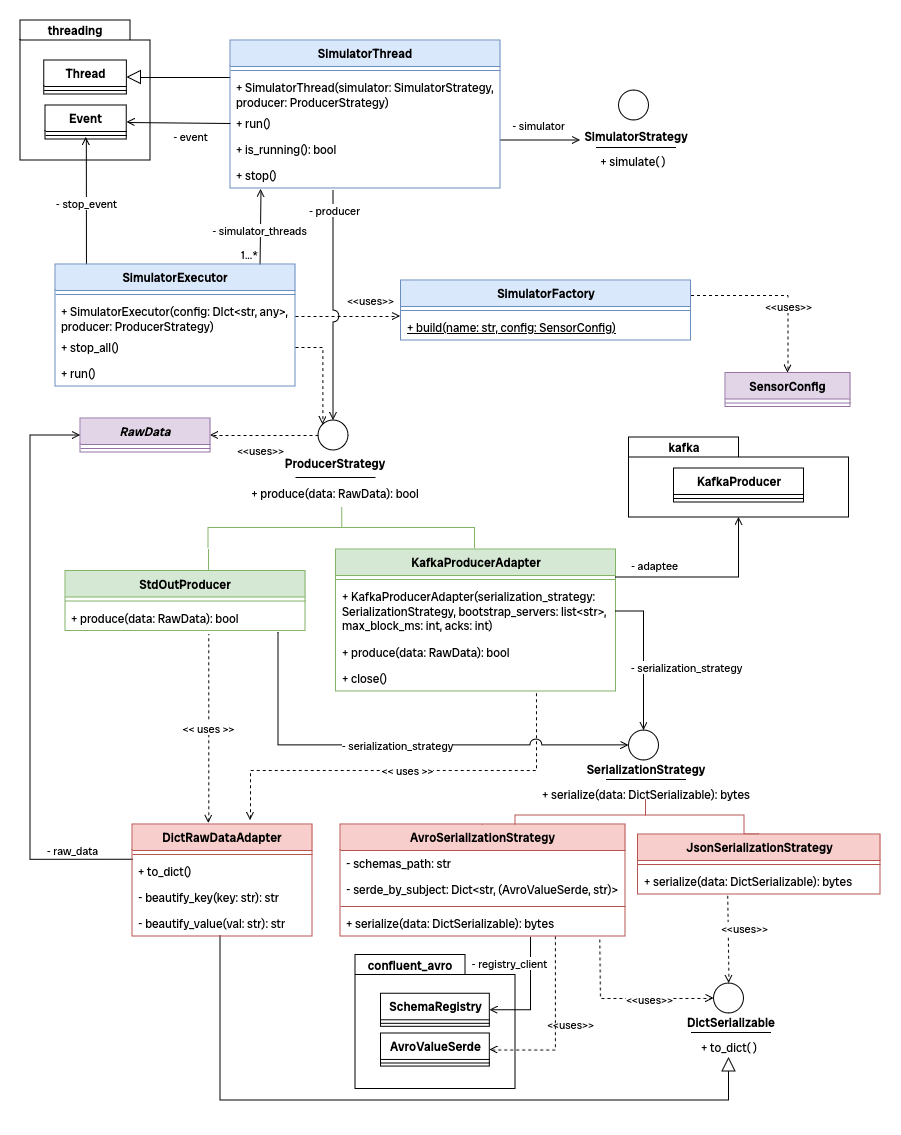
\includegraphics[width=0.87\textwidth]{./specifica_tecnica/producers_serializers.png}
	\captionof{figure}{Diagramma delle classi modulo \texttt{producers} e \texttt{serializers}}
\end{center}

\subsubsubsection{Classi, interfacce metodi e attributi}
\begin{itemize}
	\item \textbf{Interfaccia SerializationStrategy}
	      \begin{itemize}
		      \item \textbf{Metodi}:
		            \begin{itemize}
			            \item \texttt{serialize(data: DictSerializable)} bytes [public]: metodo che serializza i dati grezzi in \textit{byte}.
		            \end{itemize}
	      \end{itemize}
	\item \textbf{Interfaccia DictSerializable}
	      \begin{itemize}
		      \item \textbf{Metodi}:
		            \begin{itemize}
			            \item \texttt{to\_dict()} dict [public]: metodo che restituisce un dizionario \href{https://7last.github.io/docs/pb/documentazione-interna/glossario\#python}{Python\textsubscript{G}}.
		            \end{itemize}
	      \end{itemize}
	\item \textbf{Classe AvroSerializationStrategy}
	      \begin{itemize}
		      \item \textbf{Attributi}:
		            \begin{itemize}
			            \item \texttt{schemas\_path} str [private]: percorso della cartella contenente gli schemi Avro;
			            \item \texttt{registry\_client} SchemaRegistry [private]: client per interagire con lo \href{https://7last.github.io/docs/pb/documentazione-interna/glossario\#schema-registry}{schema registry\textsubscript{G}}, contenuto nella libreria \texttt{confluent\_avro};
			            \item \texttt{serde\_by\_subject} Dict[str, (AvroValueSerde, str)] [private]: \textit{cache} per memorizzare gli oggetti \texttt{AvroValueSerde} e gli schemi Avro associati.
		            \end{itemize}
		      \item \textbf{Metodi}:
		            \begin{itemize}
			            \item \texttt{serialize(data: DictSerializable)} bytes [public]: serializza i dati grezzi in \textit{byte} utilizzando il formato Confluent Avro.
		            \end{itemize}
	      \end{itemize}
	\item \textbf{Classe DictRawDataAdapter}
	      \begin{itemize}
		      \item \textbf{Metodi}:
		            \begin{itemize}
			            \item \texttt{to\_dict()} dict [public]: restituisce un dizionario \href{https://7last.github.io/docs/pb/documentazione-interna/glossario\#python}{Python\textsubscript{G}} a partire da un'istanza di \texttt{RawData};
			            \item \texttt{beautify\_key(key: str)} str [private]: formatta una chiave del dizionario;
			            \item \texttt{beautify\_value(value: object)} str [private]: formatta un valore del dizionario.
		            \end{itemize}
	      \end{itemize}
	\item \textbf{Classe JsonSerializationStrategy}
	      \begin{itemize}
		      \item \textbf{Metodi}:
		            \begin{itemize}
			            \item \texttt{serialize(data: DictSerializable)} bytes [public]:
		            \end{itemize}
	      \end{itemize}

\end{itemize}

\subsection{Redpanda}
\subsubsection{\textit{Topic}}
Nel contesto di \href{https://7last.github.io/docs/pb/documentazione-interna/glossario\#redpanda}{Redpanda\textsubscript{G}}, un \href{https://7last.github.io/docs/pb/documentazione-interna/glossario\#topic}{\textit{topic}\textsubscript{G}} è una categoria o canale a cui vengono inviati i dati. Essi sono utili per
organizzare logicamente i diversi tipi di messaggi o eventi. Nel nostro sistema, i dati grezzi provenienti dai simulatori vengono pubblicati in un \href{https://7last.github.io/docs/pb/documentazione-interna/glossario\#topic}{\textit{topic}\textsubscript{G}}
differente per ciascun tipo di dato; ciò consente di elaborare in modo indipendente le varie tipologie di messaggi.

\subsubsection{Partizioni e chiavi}
I \href{https://7last.github.io/docs/pb/documentazione-interna/glossario\#topic}{\textit{topic}\textsubscript{G}} possono essere suddivisi in più partizioni, le quali consentono la distribuzione del carico di lavoro tra più \href{https://7last.github.io/docs/pb/documentazione-interna/glossario\#broker}{\textit{broker}\textsubscript{G}} \href{https://7last.github.io/docs/pb/documentazione-interna/glossario\#redpanda}{Redpanda\textsubscript{G}},
allo scopo di migliorare le prestazioni e la scalabilità. Ciascuna partizione di un \href{https://7last.github.io/docs/pb/documentazione-interna/glossario\#topic}{\textit{topic}\textsubscript{G}} viene memorizzata in diversi nodi del \textit{cluster}; la numerosità
delle partizioni può essere configurata a seconda delle necessità.\\
\href{https://7last.github.io/docs/pb/documentazione-interna/glossario\#redpanda}{Redpanda\textsubscript{G}} garantisce l'ordine degli eventi all'interno della stessa partizione, tuttavia di \textit{default} non è garantito l'ordine tra partizioni diverse.
Il partizionamento consente di elaborare i dati in parallelo, infatti i consumatori possono leggere da più partizioni contemporaneamente, distribuendo il carico computazionale e migliorando il \textit{throughput}.
Ogni messaggio pubblicato è detto \textit{record} e ha una chiave, che può essere utilizzata per determinare la partizione a cui il messaggio verrà assegnato, ed un valore,
che costituisce il vero e proprio \textit{payload}; eventi con la stessa chiave vengono inviati alla stessa partizione.\\
Nel caso del nostro progetto, abbiamo deciso di utilizzare come chiave il \texttt{sensor\_uuid}, un identificativo univoco globale per ciascun \href{https://7last.github.io/docs/pb/documentazione-interna/glossario\#sensore}{sensore\textsubscript{G}}, affinché i dati
siano inviati alla stessa partizione e conseguentemente elaborati nell'ordine in cui sono stati prodotti.

\subsubsection{Redpanda \textit{schema registry}}
Lo \href{https://7last.github.io/docs/pb/documentazione-interna/glossario\#schema-registry}{\textit{schema registry}\textsubscript{G}} offre un archivio centralizzato per gestire e convalidare gli schemi associati ai messaggi Kafka, facilitandone la serializzazione e deserializzazione.
I produttori e consumatori dei \href{https://7last.github.io/docs/pb/documentazione-interna/glossario\#topic}{\textit{topic}\textsubscript{G}} Kafka possono utilizzare questi schemi per garantire coerenza e compatibilità dei dati durante la loro evoluzione nel tempo.

\subsubsubsection{\textit{Compatibility mode}}
Le modalità di compatibilità di uno schema sono delle regole che determinano come i cambiamenti ad uno schema influiscono sulla capacità dei dati serializzati con
versioni precedenti di essere letti da versioni successive e viceversa; sono essenziali per garantire che i dati rimangano compatibili durante l'evoluzione degli schemi.
Di seguito sono descritte le principali modalità di compatibilità supportate dallo \href{https://7last.github.io/docs/pb/documentazione-interna/glossario\#schema-registry}{\textit{schema registry}\textsubscript{G}} di \href{https://7last.github.io/docs/pb/documentazione-interna/glossario\#redpanda}{Redpanda\textsubscript{G}}:

\begin{itemize}
	\item \texttt{BACKWARD}: i consumatori che utilizzano lo schema più recente possono leggere i dati prodotti con lo schema precedente;
	\item \texttt{BACKWARD\_TRANSITIVE}: i consumatori che utilizzano lo schema più recente possono leggere i dati prodotti con tutti gli schemi precedenti;
	\item \texttt{FORWARD}: i consumatori che utilizzano lo schema precedente possono leggere i dati prodotti con lo schema più recente;
	\item \texttt{FORWARD\_TRANSITIVE}: i consumatori che utilizzano uno qualsiasi degli schemi precedenti possono leggere i dati prodotti con lo schema più recente;
	\item \texttt{FULL}: i dati prodotti con lo schema più recente possono essere letti da consumatori che utilizzano lo schema precedente e viceversa;
	\item \texttt{FULL\_TRANSITIVE}: i dati prodotti con uno qualsiasi degli schemi possono essere letti da consumatori che utilizzano qualsiasi altro schema;
	\item \texttt{NONE}: nessun controllo di compatibilità viene effettuato.
\end{itemize}
Nel progetto proposto da \textit{SyncLab S.r.L.} l'obiettivo principale è l'elaborazione dei dati in tempo reale piuttosto che di quelli storici, pertanto
è importante che i consumatori possano sempre ricevere i messaggi più recenti, anche se prodotti con un nuovo schema. Pertanto questo tipo di applicazioni beneficiano
della modalità \texttt{FORWARD}, ovvero quella che abbiamo scelto di utilizzare.

\subsubsubsection{Serializzazione dei dati}
\subsubsubsubsection{Chiavi}
Come menzionato in precedenza, si utilizza il \texttt{sensor\_uuid} per popolare il campo chiave dei \textit{record}; tale identificativo viene, prima di essere pubblicato
nel \href{https://7last.github.io/docs/pb/documentazione-interna/glossario\#topic}{\textit{topic}\textsubscript{G}}, convertito a stringa e codificato in UTF-8.

\subsubsubsubsection{Valori}
% TODO: parlare di Confluent Avro, del formato di serializzazione delle chiavi e partitioning strategy e di \href{https://7last.github.io/docs/pb/documentazione-interna/glossario\#topic}{topic\textsubscript{G}} name strategy <\href{https://7last.github.io/docs/pb/documentazione-interna/glossario\#topic}{topic\textsubscript{G}}>-value
Il formato Avro consente di definire attraverso \href{https://7last.github.io/docs/pb/documentazione-interna/glossario\#javascript-object-notation}{JSON\textsubscript{G}} uno schema che descriva la struttura dei dati, permettendo di serializzare e deserializzarli in modo affidabile; la serializzazione tramite
Avro produce dati binari compatti, che consentono di ridurre l'\textit{overhead} di rete e migliore le prestazioni di trasmissione dei dati.
Solamente i dati che rispettano lo schema definito possono essere inviati nel \href{https://7last.github.io/docs/pb/documentazione-interna/glossario\#topic}{\textit{topic}\textsubscript{G}}, garantendo la coerenza dei dati e facilitando la gestione delle evoluzioni dello schema.\\
Per la serializzazione dei valori abbiamo stabilito di utilizzare il formato Confluent Avro; la principale differenza rispetto al formato Avro standard è l'inclusione di un \textit{magic byte}
e dell'ID dello schema all'inizio del messaggio, seguiti dal \textit{payload} vero e proprio. Ciò consente di evitare di includere lo schema all'interno di ogni messaggio, riducendo la dimensione dei dati trasmessi.\\
Il produttore consulta lo \href{https://7last.github.io/docs/pb/documentazione-interna/glossario\#schema-registry}{\textit{schema registry}\textsubscript{G}} per ottenere l'ID corretto da utilizzare quando invia un messaggio, mentre il consumatore lo utilizza per ottenere lo schema con
cui deserializzare il messaggio.

\subsubsubsection{Formato dei messaggi}
\subsubsubsubsection{Dati grezzi prodotti dai simulatori}
Per ciascun \href{https://7last.github.io/docs/pb/documentazione-interna/glossario\#topic}{\textit{topic}\textsubscript{G}} è stato definito uno schema Avro che descrive la struttura dei dati grezzi generati dai simulatori. Rispetto all'utilizzo di uno schema comune per tutti i \href{https://7last.github.io/docs/pb/documentazione-interna/glossario\#topic}{\textit{topic}\textsubscript{G}},
questa scelta consente di:
\begin{itemize}
	\item rendere \textbf{indipendenti} i vari tipi di messaggi. Se una tipologia \href{https://7last.github.io/docs/pb/documentazione-interna/glossario\#sensore}{sensore\textsubscript{G}} dovesse cambiare il formato dei dati, sarebbe sufficiente modificare lo schema relativo al \href{https://7last.github.io/docs/pb/documentazione-interna/glossario\#topic}{\textit{topic}\textsubscript{G}} corrispondente;
	\item non dover stabilire a priori il \textbf{numero di misurazioni} che un \href{https://7last.github.io/docs/pb/documentazione-interna/glossario\#sensore}{sensore\textsubscript{G}} può effettuare. Se si utilizzasse uno schema comune, sarebbe necessario prevedere un numero massimo di campi, anche se non tutti i sensori potrebbero utilizzarli;
	\item far conoscere al consumatore il \textbf{tipo esatto} del dato che riceverà, senza dover utilizzare un campo di tipo \textit{union}. Le misurazioni effettuate dai sensori possono essere numeri interi, decimali, stringhe o booleani;
\end{itemize}
\pagebreak
I sensori inviano, oltre alle misurazioni relative alla propria tipologia, i campi contenuti nella seguente tabella:
\begin{table}[ht]
	\begin{tabular}{lll}
		\textbf{Campo}        & \textbf{Tipo} & \textbf{Descrizione}                                     \\
		\texttt{sensor\_uuid} & string        & Identificativo univoco del \href{https://7last.github.io/docs/pb/documentazione-interna/glossario\#sensore}{sensore\textsubscript{G}}.                      \\
		\texttt{sensor\_name} & string        & Nome del \href{https://7last.github.io/docs/pb/documentazione-interna/glossario\#sensore}{sensore\textsubscript{G}}.                                        \\
		\texttt{latitude}     & double        & Latitudine del \href{https://7last.github.io/docs/pb/documentazione-interna/glossario\#sensore}{sensore\textsubscript{G}}.                                  \\
		\texttt{longitude}    & double        & Longitudine del \href{https://7last.github.io/docs/pb/documentazione-interna/glossario\#sensore}{sensore\textsubscript{G}}.                                 \\
		\texttt{timestamp}    & string        & Data e ora della misurazione in formato ISO 8601.        \\
		\texttt{group\_name}  & string        & Nome (opzionale) del gruppo di sensori a cui appartiene. \\
	\end{tabular}
\end{table}
\\
Un esempio di schema Avro per il tipo di dato \texttt{Temperature} è il seguente:
\begin{lstlisting}[language=json, caption=Esempio di schema Avro per il tipo di dato \texttt{Temperature},captionpos=b]
{
  "type": "record",
  "name": "Temperature",
  "fields": [
    { "name": "sensor_uuid", "type": "string" },
    { "name": "sensor_name", "type": "string" },
    { "name": "latitude", "type": "double" },
    { "name": "longitude", "type": "double" },
    { "name": "timestamp", "type": "string" },
    { "name": "value", "type": "float" },
    { "name": "group_name", "type": [ "string", "null" ] }
  ]
}
\end{lstlisting}

\subsubsubsubsection{Dati elaborati da Apache Flink}
Per quanto riguarda invece i dati aggregati da Apache Flink, è stato definito uno schema Avro per ciascuno di essi, il quale viene pubblicato in un \href{https://7last.github.io/docs/pb/documentazione-interna/glossario\#topic}{\textit{topic}\textsubscript{G}} dedicato.
Lo schema Avro per il tipo di dato \texttt{HeatIndex} è il seguente:
\begin{lstlisting}[language=json, caption=Schema Avro per il tipo di dato \texttt{HeatIndex},captionpos=b]
{
  "type": "record",
  "name": "Heat_Index",
  "fields": [
    {"name":"sensor_names", "type": {"type":"array", "items":"string"}},
    {"name":"group_name", "type": "string"},
    {"name":"heat_index", "type": "float"},
    {"name":"avg_temperature", "type": "float"},
    {"name":"avg_humidity", "type": "float"},
    {"name":"center_of_mass_latitude", "type": "float"},
    {"name":"center_of_mass_longitude", "type": "float"},
    {"name":"radius_in_km", "type": "float"},
    {"name":"timestamp", "type": "string"}
  ]
}

\end{lstlisting}

\begin{lstlisting}[language=json, caption=Schema Avro per il tipo di dato \texttt{ChargingEfficiency},captionpos=b]
{
  "type": "record",
  "name": "Charging_Efficiency",
  "fields": [
    { "name": "sensor_uuid", "type": "string" },
    { "name": "utilization_rate", "type": "double" },
    { "name": "efficiency_rate", "type": "double" },
    { "name": "timestamp", "type": "string" },
    { "name": "group_name", "type": "string" },
    { "name":"sensor_names", "type": { "type": "array",  "items": "string" } }
  ]
}

\end{lstlisting}

\subsubsubsection{Altre configurazioni}
\begin{itemize}
	\item \textbf{Numero di partizioni}: il numero di partizioni di un \href{https://7last.github.io/docs/pb/documentazione-interna/glossario\#topic}{\textit{topic}\textsubscript{G}} è stato configurato con \textit{default} a 3;
	\item \textit{Subject name strategy}, ovvero la strategia per la generazione del nome dello schema all'interno dello \href{https://7last.github.io/docs/pb/documentazione-interna/glossario\#schema-registry}{\textit{schema registry}\textsubscript{G}}, è stata impostata a \texttt{TopicNameStrategy},
	      che prevede che il nome dello schema sia composto dal nome del \href{https://7last.github.io/docs/pb/documentazione-interna/glossario\#topic}{\textit{topic}\textsubscript{G}} seguito da \texttt{-value} per i valori e \texttt{-key} per le chiavi.
\end{itemize}

\subsubsection{Inizializzazione e configurazione}
Apache Flink necessita che i \href{https://7last.github.io/docs/pb/documentazione-interna/glossario\#topic}{\textit{topic}\textsubscript{G}} da cui consuma, ovvero temperatura, umidità, colonnine di ricarica e parcheggi, e quelli in cui pubblica, ovvero \texttt{heat\_index} e \\\texttt{charging\_efficiency},
siano creati precedentemente all'esecuzione del \href{https://7last.github.io/docs/pb/documentazione-interna/glossario\#job}{\textit{job}\textsubscript{G}}, con i rispettivi schemi. A tale scopo, è stata realizzata un'immagine \href{https://7last.github.io/docs/pb/documentazione-interna/glossario\#docker}{Docker\textsubscript{G}} basata su \href{https://hub.docker.com/_/alpine}{\underline{Alpine Linux}} [Ultima consultazione 2024-07-18],
al cui interno viene scaricato il binario \href{https://docs.redpanda.com/current/get-started/intro-to-rpk/}{\underline{rpk}} [Ultima consultazione 2024-07-18], strumento
messo a disposizione da \href{https://7last.github.io/docs/pb/documentazione-interna/glossario\#redpanda}{Redpanda\textsubscript{G}} per interagire e configurare un \textit{cluster} \href{https://7last.github.io/docs/pb/documentazione-interna/glossario\#redpanda}{Redpanda\textsubscript{G}}, anche remoto. Al suo interno inoltre è presente uno \textit{script} Bash che
dato il nome di un \href{https://7last.github.io/docs/pb/documentazione-interna/glossario\#topic}{\textit{topic}\textsubscript{G}} lo crea se non esiste e ne registra lo schema all'interno dello \href{https://7last.github.io/docs/pb/documentazione-interna/glossario\#schema-registry}{\textit{schema registry}\textsubscript{G}}.

\subsubsection{Redpanda Connect}\label{redpanda_connect}
\href{https://7last.github.io/docs/pb/documentazione-interna/glossario\#redpanda}{Redpanda\textsubscript{G}} Connect è una piattaforma integrata nel sistema \href{https://7last.github.io/docs/pb/documentazione-interna/glossario\#redpanda}{Redpanda\textsubscript{G}}, progettata per facilitare l'integrazione e il trasferimento dei dati tra \href{https://7last.github.io/docs/pb/documentazione-interna/glossario\#redpanda}{Redpanda\textsubscript{G}} e altre fonti o destinazioni.
Esso consente di gestire dei connettori, componenti \textit{software} che si occupano automatizzare lo spostamento dei dati da e verso \href{https://7last.github.io/docs/pb/documentazione-interna/glossario\#redpanda}{Redpanda\textsubscript{G}}. Tali connettori si dividono in due categorie:
\begin{itemize}
	\item \textbf{\textit{source connector}}: si occupano di trasferire i dati da una sorgente esterna a \href{https://7last.github.io/docs/pb/documentazione-interna/glossario\#redpanda}{Redpanda\textsubscript{G}};
	\item \textbf{\textit{sink connector}}: si occupano di trasferire i dati da \href{https://7last.github.io/docs/pb/documentazione-interna/glossario\#redpanda}{Redpanda\textsubscript{G}} a una destinazione esterna.
\end{itemize}

\subsubsubsection{\textit{Sink connector} per \href{https://7last.github.io/docs/pb/documentazione-interna/glossario\#clickhouse}{ClickHouse\textsubscript{G}}}
All'interno del progetto abbiamo utilizzato \href{https://7last.github.io/docs/pb/documentazione-interna/glossario\#redpanda}{Redpanda\textsubscript{G}} Connect per persistere su \href{https://7last.github.io/docs/pb/documentazione-interna/glossario\#clickhouse}{ClickHouse\textsubscript{G}} i dati provenienti dai sensori pubblicati nei differenti \href{https://7last.github.io/docs/pb/documentazione-interna/glossario\#topic}{\textit{topic}\textsubscript{G}}. Per
poter effettuare questa operazione è stato necessario utilizzare un \textit{sink connector}, che si occupasse di deserializzare i messaggi in formato Confluent Avro, effettuare
il \textit{parsing} dei campi di tipo \texttt{DateTime} (pubblicati come stringhe in formato \href{https://www.iso.org/iso-8601-date-and-time-format.html}{\underline{ISO 8601}})
ed infine salvare i dati in \href{https://7last.github.io/docs/pb/documentazione-interna/glossario\#clickhouse}{ClickHouse\textsubscript{G}}.\\
La documentazione relativa è consultabile al seguente \href{https://clickhouse.com/docs/en/integrations/kafka/clickhouse-kafka-connect-sink}{\underline{url}}
[Ultima consultazione 2024-07-10].\\
La configurazione di tale connettore è disponibile all'interno del \textit{repository} del progetto al percorso \href{https://7last.github.io/docs/pb/documentazione-interna/glossario\#redpanda}{\texttt{redpanda}\textsubscript{G}}\texttt{/connectors/configs/\href{https://7last.github.io/docs/pb/documentazione-interna/glossario\#clickhouse}{clickhouse\textsubscript{G}}.\href{https://7last.github.io/docs/pb/documentazione-interna/glossario\#javascript-object-notation}{json\textsubscript{G}}}.
Al fine di effettuare il \textit{parsing} delle date è stato necessario definire all'interno di tale file un \textit{transformer}, il quale si occupa di leggere il campo \texttt{timestamp}
e convertirlo in \texttt{DateTime}, tipo riconosciuto da \href{https://7last.github.io/docs/pb/documentazione-interna/glossario\#clickhouse}{ClickHouse\textsubscript{G}}.\\
La versione utilizzata è la 1.1.1, scaricabile dal seguente \href{https://github.com/ClickHouse/clickhouse-kafka-connect/releases}{\underline{url}} [Ultima consultazione 2024-07-10].\\
La configurazione del \textit{transformer} è la seguente:
\mySkip{\begin{lstlisting}[language=json, caption=Configurazione del \textit{transformer} all'interno del file \href{https://7last.github.io/docs/pb/documentazione-interna/glossario\#clickhouse}{\texttt{clickhouse}\textsubscript{G}}\texttt{.\href{https://7last.github.io/docs/pb/documentazione-interna/glossario\#javascript-object-notation}{json\textsubscript{G}}},captionpos=b]
{
    //...
    "transforms": "TimestampConverter",
    "transforms.TimestampConverter.type": "org.apache.kafka.connect.transforms.TimestampConverter$Value",
    "transforms.TimestampConverter.format": "yyyy-MM-dd'T'HH:mm:ss",
    "transforms.TimestampConverter.field": "timestamp",
    "transforms.TimestampConverter.target.type": "Timestamp"
    //...
}
\end{lstlisting}}
La creazione del connettore viene effettuata eseguendo il seguente comando nella radice del progetto:
\begin{verbatim}
curl "localhost:8083/connectors" -H 'Content-Type: application/\href{https://7last.github.io/docs/pb/documentazione-interna/glossario\#javascript-object-notation}{json\textsubscript{G}}' \
    -d @./\href{https://7last.github.io/docs/pb/documentazione-interna/glossario\#redpanda}{redpanda\textsubscript{G}}/connectors/configs/\href{https://7last.github.io/docs/pb/documentazione-interna/glossario\#clickhouse}{clickhouse\textsubscript{G}}.\href{https://7last.github.io/docs/pb/documentazione-interna/glossario\#javascript-object-notation}{json\textsubscript{G}}
\end{verbatim}

\subsubsubsection{Avro converter}
È stato inoltre necessario utilizzare un ulteriore \textit{plugin}, \texttt{avro-converter} (versione 7.6.1), scaricabile dal seguente
\href{https://www.confluent.io/hub/confluentinc/kafka-connect-avro-converter}{\underline{url}} [Ultima consultazione 2024-07-10],
il quale consente di effettuare la deserializzazione dei messaggi in formato Confluent Avro.\\
Il \textit{connector sink} è stato configurato per utilizzarlo come segue:
\begin{lstlisting}[language=json, caption=Utilizzo del \textit{plugin} \texttt{avro-converter} all'interno del file \href{https://7last.github.io/docs/pb/documentazione-interna/glossario\#clickhouse}{\texttt{clickhouse}\textsubscript{G}}\texttt{.\href{https://7last.github.io/docs/pb/documentazione-interna/glossario\#javascript-object-notation}{json\textsubscript{G}}},captionpos=b]
{
    //...
    "value.converter": "io.confluent.connect.avro.AvroConverter",
    "value.converter.schemas.enable": "true",
    "value.converter.schema.registry.url": "http://redpanda:8081"
    //...
}
\end{lstlisting}

\subsubsection{Redpanda Console}
\href{https://7last.github.io/docs/pb/documentazione-interna/glossario\#redpanda}{Redpanda\textsubscript{G}} Console è un'applicazione web che consente di gestire e effettuare \textit{debug} di un'istanza \href{https://7last.github.io/docs/pb/documentazione-interna/glossario\#redpanda}{Redpanda\textsubscript{G}}. Essa ha diverse funzionalità, tra cui:
%
\begin{itemize}
	\item \textbf{visualizzazione dei messaggi}: consente di esplorare i messaggi dei \href{https://7last.github.io/docs/pb/documentazione-interna/glossario\#topic}{\textit{topic}\textsubscript{G}} attraverso \textit{query} ad-hoc e filtri dinamici, scritti con semplici funzioni JavaScript;
	\item \textbf{gruppi di consumatori}: permette di visualizzare tutti i gruppi di consumatori attivi, insieme ai relativi offset, modificarli o eliminarli;
	\item \textbf{panoramica dei \href{https://7last.github.io/docs/pb/documentazione-interna/glossario\#topic}{\textit{topic}\textsubscript{G}}}: permette di visualizzare la lista dei \href{https://7last.github.io/docs/pb/documentazione-interna/glossario\#topic}{\textit{topic}\textsubscript{G}}, controllarne la configurazione, lo spazio utilizzato, la lista dei consumatori e i dettagli delle partizioni;
	\item \textbf{panoramica del \textit{cluster}}: permette di visualizzare le ACL, i \href{https://7last.github.io/docs/pb/documentazione-interna/glossario\#broker}{\textit{broker}\textsubscript{G}} disponibili, il loro spazio utilizzato, l'ID del rack e altre informazioni per ottenere una panoramica del \textit{cluster};
	\item \href{https://7last.github.io/docs/pb/documentazione-interna/glossario\#schema-registry}{\textbf{\textit{schema registry}}\textsubscript{G}}: permette di visualizzare tutti gli schemi Avro, Protobuf o \href{https://7last.github.io/docs/pb/documentazione-interna/glossario\#javascript-object-notation}{JSON\textsubscript{G}} all'interno del registro degli schemi;
	\item \textbf{Kafka Connect}: permette di gestire i connettori da più \textit{cluster} di connessione, modificare le configurazioni, visualizzare lo stato corrente o riavviare i task.
\end{itemize}

\subsection{Apache Flink - \textit{Processing layer}}
Nel contesto di Apache Flink, un \href{https://7last.github.io/docs/pb/documentazione-interna/glossario\#job}{\textit{job}\textsubscript{G}} è un'applicazione che definisce una serie di operazioni di trasformazione su un flusso di dati.
Essi possono essere eseguiti su \textit{cluster} distribuiti per sfruttare la scalabilità e la potenza di calcolo necessaria per elaborare grandi quantità di dati in tempo reale.
Tipicamente, un \href{https://7last.github.io/docs/pb/documentazione-interna/glossario\#job}{\textit{job}\textsubscript{G}} consiste di tre componenti principali:
\begin{itemize}
	\item \textbf{sorgente di dati (\textit{source})}: il punto di ingresso del flusso di dati, ad esempio un \href{https://7last.github.io/docs/pb/documentazione-interna/glossario\#topic}{\textit{topic}\textsubscript{G}} Kafka o un file di log;
	\item \textbf{transformations}: operazioni come map, filter, aggregate, join, che trasformano i dati in ingresso;
	\item \textbf{\textit{sink}}: il punto di uscita dove i dati elaborati vengono scritti, ad esempio un database o un altro \href{https://7last.github.io/docs/pb/documentazione-interna/glossario\#topic}{\textit{topic}\textsubscript{G}} Kafka.
\end{itemize}
Flink offre due API per la definizione dei \href{https://7last.github.io/docs/pb/documentazione-interna/glossario\#job}{\textit{job}\textsubscript{G}}: \textit{DataStream API} e \textit{Table API}
Il primo consente di lavorare con \textit{stream} di dati, avendo un controllo più fine sul flusso di dati, mentre il secondo permette di lavorare con tabelle, offrendo una sintassi più simile a SQL.\\
Per questo progetto abbiamo utilizzato le \textit{DataStream API} per la realizzazione di due \href{https://7last.github.io/docs/pb/documentazione-interna/glossario\#job}{\textit{job}\textsubscript{G}} indipendenti tra loro, che tuttavia condividono alcune classi di utilità.

\subsubsection{\textit{Watermark}}\label{watermark}
I \textit{watermark} sono un meccanismo che Flink utilizza per tracciare l'avanzamento del tempo degli eventi
(il tempo in cui gli eventi si sono effettivamente verificati nel mondo reale, rispetto al tempo in cui gli eventi vengono elaborati dal sistema)
per un flusso di dati. I \textit{watermark} non sono necessari in tutti gli scenari di elaborazione dei flussi,
ma quando vengono utilizzati sono emessi da Flink nel flusso di dati di origine.
Non si tratta di eventi di dati veri e propri, ma di marcatori di metadati utilizzati per tracciare l'aspetto temporale del flusso durante l'elaborazione degli eventi.\\
In un flusso di dati, un \textit{watermark} indica che non devono arrivare altri eventi più vecchi del timestamp del \textit{watermark} stesso,
trasmettendo l'informazione di completezza dei dati fino a quel momento.
I \textit{watermark} hanno diversi scopi fondamentali in Apache Flink:
\begin{itemize}
	\item consentono a Flink di elaborare i flussi di dati in base all'ora di produzione dell'evento piuttosto che quella di elaborazione e consentono a Flink
	      di tracciare la progressione dell'ora dell'evento per ogni sorgente di dati. Questo è particolarmente importante quando gli eventi arrivano fuori ordine,
	      poiché i \textit{watermark} assicurano che Flink elabori gli eventi nell'ordine corretto in base ai loro timestamp;
	\item sono fondamentali per le operazioni basate sul tempo, come l'utilizzo di funzioni di \textit{window}, che consentono di raggruppare gli eventi in finestre temporali
	      e calcolare risultati basati su tali finestre. Flink utilizza i \textit{watermark} per determinare quando attivare i calcoli delle finestre ed emettere i risultati delle stesse;
	\item aiutano Flink a rilevare gli eventi in ritardo, cioè quelli che arrivano dopo un \textit{watermark}, in termini di tempo.
	      Tracciando i \textit{watermark}, Flink può permettere all'applicazione di decidere se ignorare o elaborare tali eventi e per quanto tempo continuare ad accettare dati in ritardo.
\end{itemize}
All'interno dei due \href{https://7last.github.io/docs/pb/documentazione-interna/glossario\#job}{\textit{job}\textsubscript{G}} implementati abbiamo assegnato i \textit{watermark} ammettendo un ritardo massimo di 10 secondi. Il \textit{timestamp} considerato per
ciascun evento è quello relativo al campo \texttt{timestamp} presente nei dati grezzi prodotti dai simulatori e dunque non considera il tempo di elaborazione ma quello di produzione del dato.

\subsubsubsection{\textit{Heat Index}}
A partire dai dati rilevati dai sensori di temperatura e umidità relativa lo \href{https://7last.github.io/docs/pb/documentazione-interna/glossario\#heat-index}{\textit{Heat Index}\textsubscript{G}} consente di stimare la percezione della temperatura da parte dell'essere umano.
Nella configurazione di ciascun simulatore, oltre a posizione e identificativo dello stesso, è possibile specificare un \texttt{group\_name}, ovvero una stringa che identifica
il gruppo o zona di appartenenza; si suppone che sensori situati in posizioni geografiche vicine abbiano lo stesso \texttt{group\_name}. Il \href{https://7last.github.io/docs/pb/documentazione-interna/glossario\#job}{\textit{job}\textsubscript{G}} calcola prima separatamente
la temperatura e l'umidità media per finestre di un'ora, aggregando i dati provenienti da sensori dello stesso gruppo. Successivamente con i valori ottenuti computa lo \href{https://7last.github.io/docs/pb/documentazione-interna/glossario\#heat-index}{\textit{Heat Index}\textsubscript{G}},
utilizzando la \\\underline{\href{https://www.ncbi.nlm.nih.gov/pmc/articles/PMC3801457/}{formula empirica ideata da Blazejczyk}} [Ultima consultazione 2024-06-25].
Nel risultato finale, oltre al valore dello \href{https://7last.github.io/docs/pb/documentazione-interna/glossario\#heat-index}{\textit{Heat Index}\textsubscript{G}}, vengono restituiti anche i valori di temperatura e umidità medi, il \href{https://7last.github.io/docs/pb/documentazione-interna/glossario\#centro-di-massa}{centro di massa\textsubscript{G}} del gruppo di sensori
(utilizzando la formula \underline{\href{https://en.wikipedia.org/wiki/Haversine_formula}{Haversine}} [Ultima consultazione 2024-06-25] per il calcolo della distanza) e la
distanza dal \href{https://7last.github.io/docs/pb/documentazione-interna/glossario\#centro-di-massa}{centro di massa\textsubscript{G}} al \href{https://7last.github.io/docs/pb/documentazione-interna/glossario\#sensore}{sensore\textsubscript{G}} più lontano. Questi ultimi due dati sono impiegati in una mappa interattiva su \href{https://7last.github.io/docs/pb/documentazione-interna/glossario\#grafana}{Grafana\textsubscript{G}} per poter disegnare un cerchio,
rappresentante la zona di influenza del gruppo di sensori.

\subsubsubsubsection{Modello di calcolo}
\subsubsubsubsubsection{Heat Index}
Lo \href{https://7last.github.io/docs/pb/documentazione-interna/glossario\#heat-index}{\textit{Heat Index}\textsubscript{G}} viene calcolato con la seguente formula, dove $T$ è la temperatura in gradi Celsius, $R$ l'umidità relativa in percentuale:
\[
	HI = c_1 + c_2 T + c_3 R + c_4 TR + c_5 T^2 + c_6 R^2 + c_7 T^2 R + c_8 TR^2 + c_9 T^2 R^2
\]
e i coefficienti $c_i$ sono:
\begin{align*}
	c_1 & = -8.78469475556          & \quad c_2 & = 1.61139411            & \quad c_3 & = 2.33854883889         \\
	c_4 & = -0.14611605             & \quad c_5 & = -0.012308094          & \quad c_6 & = -0.0164248277778      \\
	c_7 & = 2.211732 \times 10^{-3} & \quad c_8 & = 7.2546 \times 10^{-4} & \quad c_9 & = -3.582 \times 10^{-6}
\end{align*}
\subsubsubsubsubsection{Centro di massa o centroide}
Il calcolo del \href{https://7last.github.io/docs/pb/documentazione-interna/glossario\#centro-di-massa}{centro di massa\textsubscript{G}} tiene in considerazione la sfericità della Terra. Sia dato un insieme di punti $P = \{(a_1, b_1), (a_2, b_2), \ldots, (a_n, b_n)\}$, dove $a_i$ rappresenta
la latitudine del punto $i$-esimo e $b_i$ la longitudine. Per calcolare il \href{https://7last.github.io/docs/pb/documentazione-interna/glossario\#centro-di-massa}{centro di massa\textsubscript{G}} si procede, per ciascun punto, a convertire in radianti le coordinate:
\begin{align*}
	\mySkip{lat}_i = \frac{\pi}{180} \cdot a_i, & \quad \mySkip{lon}_i = \frac{\pi}{180} \cdot b_i
\end{align*}
Successivamente si calcolano i coefficienti $x_i$, $y_i$ e $z_i$:
\begin{align*}
	x_i = \cos(\mySkip{lat}_i) \cdot \cos(\mySkip{lon}_i),       &
	\quad y_i = \cos(\mySkip{lat}_i) \cdot \sin(\mySkip{lon}_i), &
	\quad z_i = \sin(\mySkip{lat}_i)
\end{align*}
Una volta ottenuti i coefficienti per tutti i punti, si calcola la media di tutti i coefficienti:
\begin{align*}
	x & = \frac{1}{n} \sum_{i=1}^{n} x_i, & \quad y = \frac{1}{n} \sum_{i=1}^{n} y_i, & \quad z = \frac{1}{n} \sum_{i=1}^{n} z_i
\end{align*}

Infine si calcolano $\mySkip{lat}$ (latitudine in radianti), $\mySkip{lon}$ (longitudine in radianti) e $\mySkip{hyp}$ (ipotenusa ne piano cartesiano, che rappresenta la distanza dall'origine alla proiezione del punto sul piano $\mySkip{lat}_i, \mySkip{lon}_i$):
\begin{align*}
	\mySkip{lon} = \mySkip{atan2}(y, x) \\
	\mySkip{hyp} = \sqrt{x^2 + y^2}     \\
	\mySkip{lat} = \mySkip{atan2}(z, \mySkip{hyp})
\end{align*}
Una volta ottenuti $\mySkip{lat}$ e $\mySkip{lon}$, si convertono in gradi e si ottiene il \href{https://7last.github.io/docs/pb/documentazione-interna/glossario\#centro-di-massa}{centro di massa\textsubscript{G}} $CM = (c_a, c_b)$.
\begin{align*}
	c_a = \frac{180}{\pi} \cdot \mySkip{lat}, & \quad c_b = \frac{180}{\pi} \cdot \mySkip{lon}
\end{align*}
\subsubsubsubsubsection{Raggio del cerchio}
Il raggio del cerchio viene calcolato come la distanza dal \href{https://7last.github.io/docs/pb/documentazione-interna/glossario\#centro-di-massa}{centro di massa\textsubscript{G}} al punto più lontano. Sia $P = \{(a_1, b_1), (a_2, b_2), \ldots, (a_n, b_n)\}$ l'insieme di punti, $CM = (c_a, c_b)$, il
raggio $r$ è dato da:
\[
	r = \max_{i=1}^{n} haversine(c_a, c_b, a_i, b_i)
\]


\subsubsubsubsection{Flusso di dati}
\begin{center}
	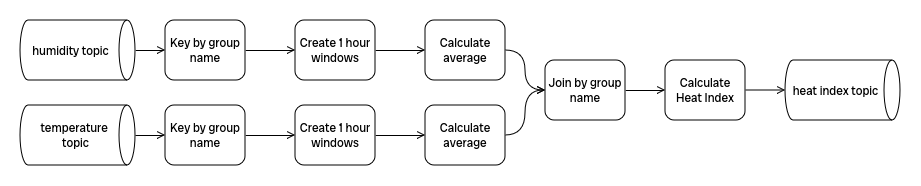
\includegraphics[width=1\textwidth]{./specifica_tecnica/heat_index_flow.png}
	\captionof{figure}{Flusso di dati del \href{https://7last.github.io/docs/pb/documentazione-interna/glossario\#job}{\textit{job}\textsubscript{G}} \href{https://7last.github.io/docs/pb/documentazione-interna/glossario\#heat-index}{\textit{Heat Index}\textsubscript{G}}}
\end{center}
I seguenti passaggi vengono eseguiti indipentendemente ed in parallelo per i dati provenienti dai \href{https://7last.github.io/docs/pb/documentazione-interna/glossario\#topic}{\textit{topic}\textsubscript{G}} di temperatura ed umidità:
\begin{enumerate}
	\item lettura dei dati grezzi dai \href{https://7last.github.io/docs/pb/documentazione-interna/glossario\#topic}{\textit{topic}\textsubscript{G}} relativi alla temperatura e all'umidità, attraverso la classe \texttt{KafkaSource};
	\item assegnazione di un \textit{watermark} ai dati, come precedentemente descritto nel paragrafo \hyperref[watermark]{\underline{\textit{watermark}}};
	\item raggruppamento di dati utilizzando come chiave il \texttt{group\_name}, tramite la funzione \texttt{\mySkip{keyBy}} fornita da Flink;
	\item creazione di una finestra temporale di un'ora, utilizzando la funzione \texttt{window} di Flink;
	\item calcolo della media della temperatura e dell'umidità, utilizzando la classe \\\texttt{AverageWindowFunction};
\end{enumerate}
Successivamente, attraverso l'utilizzo dell'operatore \texttt{join} si uniscono i due \textit{stream} di dati, calcolando
attraverso la classe \texttt{HeatIndexJoinFunction} il valore dello \href{https://7last.github.io/docs/pb/documentazione-interna/glossario\#heat-index}{\textit{Heat Index}\textsubscript{G}}, la latitudine e longitudine del \href{https://7last.github.io/docs/pb/documentazione-interna/glossario\#centro-di-massa}{centro di massa\textsubscript{G}} e il raggio del cerchio.
Infine, i dati vengono pubblicati nel \href{https://7last.github.io/docs/pb/documentazione-interna/glossario\#topic}{\textit{topic}\textsubscript{G}} dedicato allo \href{https://7last.github.io/docs/pb/documentazione-interna/glossario\#heat-index}{\textit{Heat Index}\textsubscript{G}}.

\subsubsubsubsection{Architettura}
Al fine di realizzare un \href{https://7last.github.io/docs/pb/documentazione-interna/glossario\#job}{\textit{job}\textsubscript{G}}, è necessario implementare una classe dotata di un metodo \texttt{main} che si occupi di inizializzare l'ambiente di esecuzione, definire
sorgente e \textit{sink} dei dati e infine di far partire il \href{https://7last.github.io/docs/pb/documentazione-interna/glossario\#job}{\textit{job}\textsubscript{G}} vero e proprio.
La classe che svolge tale ruolo per il \href{https://7last.github.io/docs/pb/documentazione-interna/glossario\#job}{\textit{job}\textsubscript{G}} \href{https://7last.github.io/docs/pb/documentazione-interna/glossario\#heat-index}{\textit{Heat Index}\textsubscript{G}} è \texttt{HeatIndexJob}, che definisce come sorgente di dati
i \href{https://7last.github.io/docs/pb/documentazione-interna/glossario\#topic}{\textit{topic}\textsubscript{G}} relativi alla temperatura e all'umidità, leggendo le variabili d'ambiente relative all'indirizzo del \textit{bootstrap server} e \href{https://7last.github.io/docs/pb/documentazione-interna/glossario\#schema-registry}{\textit{schema registry}\textsubscript{G}},
applica le trasformazioni illustrate nel paragrafo precedente ed infine pubblica i risultati nel \href{https://7last.github.io/docs/pb/documentazione-interna/glossario\#topic}{\textit{topic}\textsubscript{G}} dedicato allo \href{https://7last.github.io/docs/pb/documentazione-interna/glossario\#heat-index}{\textit{Heat Index}\textsubscript{G}}.
In tale classe viene definito un metodo \texttt{execute}, il quale applica le trasformazioni a partire dai \textit{source} definiti nel metodo \textit{main}. Separare
la logica di esecuzione del \href{https://7last.github.io/docs/pb/documentazione-interna/glossario\#job}{\textit{job}\textsubscript{G}} dalla sua definizione consente di rendere il codice più modulare e rende possibile la realizzazione di test di integrazione sull'esecuzione
dell'intero \href{https://7last.github.io/docs/pb/documentazione-interna/glossario\#job}{\textit{job}\textsubscript{G}}, fornendo una versione \textit{mock} di \textit{source} e \textit{sink} di dati.\\
Come illustrato nel diagramma seguente, per ciascuna fase di elaborazione dei dati viene definita una classe che estende la funzione appropriata per il tipo di operazione che si
vuole effettuare. Per i casi più semplici sarebbe possibile utilizzare direttamente delle classi anonime o funzioni \textit{lambda}, tuttavia definendo classi separate
per ciascuna trasformazione consente di sottoporre ciascuna di esse a test di unità e riutilizzarle se necessario; la funzione \texttt{AverageWindowFunction} viene ad esempio
utilizzata sia per calcolare la media della temperatura che dell'umidità.

\begin{center}
	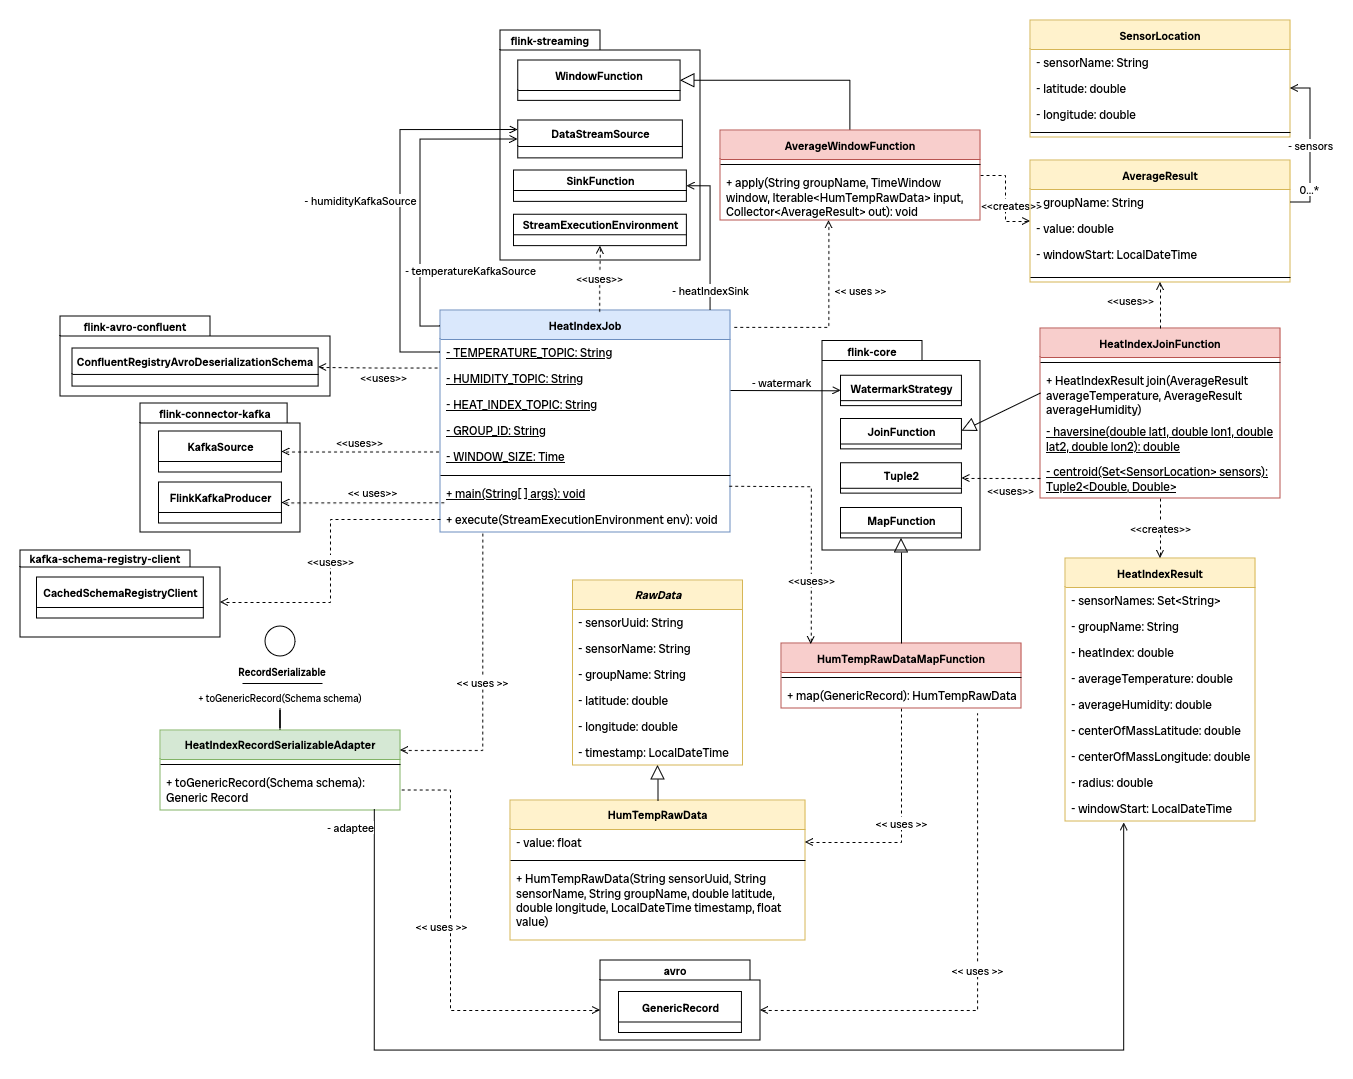
\includegraphics[width=1\textwidth]{./specifica_tecnica/heat_index_job.png}
	\captionof{figure}{Architettura del \href{https://7last.github.io/docs/pb/documentazione-interna/glossario\#job}{\textit{job}\textsubscript{G}} \href{https://7last.github.io/docs/pb/documentazione-interna/glossario\#heat-index}{\textit{Heat Index}\textsubscript{G}}}
\end{center}

\subsubsubsubsubsection{\textit{Object adapter}}\label{object_adapter}
Data la necessità di convertire la classe \texttt{HeatIndexResult}, prodotto delle aggregazioni, in un oggetto di tipo \texttt{GenericRecord} (contenuto nella libreria \texttt{avro}),
abbiamo implementato il \textit{pattern} \textit{object adapter}, che si occupa di effettuare tale conversione.\\
A tale scopo, è stata definita un'interfaccia \texttt{RecordSerializable} che espone il metodo \texttt{toGenericRecord}, il quale restituisce un oggetto di tipo \texttt{GenericRecord}.\\
\texttt{HeatIndexRecordSerializableAdapter} implementa tale interfaccia e ha un campo \\\texttt{adaptee} di tipo \texttt{HeatIndexResult}. Prima di effettuare dunque il \textit{sink}
dei dati, viene invocato il metodo \texttt{toGenericRecord} per ottenere il \textit{record} da pubblicare nel \href{https://7last.github.io/docs/pb/documentazione-interna/glossario\#topic}{\textit{topic}\textsubscript{G}} dedicato allo \href{https://7last.github.io/docs/pb/documentazione-interna/glossario\#heat-index}{\textit{Heat Index}\textsubscript{G}}.

\subsubsubsubsubsection{Classi, interfacce metodi e attributi}
\begin{itemize}
	\item \textbf{Classe HeatIndexJob}
	      \begin{itemize}
		      \item \textbf{Attributi}
		            \begin{itemize}
			            \item \texttt{TEMPERATURE\_TOPIC} str [private,final,static]: nome del \href{https://7last.github.io/docs/pb/documentazione-interna/glossario\#topic}{\textit{topic}\textsubscript{G}} relativo alla temperatura;
			            \item \texttt{HUMIDITY\_TOPIC} str [private,final,static]: nome del \href{https://7last.github.io/docs/pb/documentazione-interna/glossario\#topic}{\textit{topic}\textsubscript{G}} relativo all'umidità;
			            \item \texttt{HEAT\_INDEX\_TOPIC} str [private,final,static]: nome del \href{https://7last.github.io/docs/pb/documentazione-interna/glossario\#topic}{\textit{topic}\textsubscript{G}} relativo allo \href{https://7last.github.io/docs/pb/documentazione-interna/glossario\#heat-index}{\textit{Heat Index}\textsubscript{G}};
			            \item \texttt{GROUP\_ID} str [private,final,static]: identificativo del gruppo di consumatori;
			            \item \texttt{WINDOW\_SIZE} int [private,final,static]: dimensione della finestra temporale per cui calcolare le aggregazioni.
		            \end{itemize}
		      \item \textbf{Metodi}
		            \begin{itemize}
			            \item \texttt{main(String[] \mySkip{args})} [public,static]: metodo principale che si occupa di inizializzare l'ambiente di esecuzione, definire sorgente e \textit{sink} dei dati ed eseguire il \href{https://7last.github.io/docs/pb/documentazione-interna/glossario\#job}{\textit{job}\textsubscript{G}} vero e proprio;

			            \item \texttt{execute(StreamExecutionEnvironment \mySkip{env})} [public]: metodo che applica le trasformazioni a partire dai \textit{source} definiti nel metodo \textit{main}.
		            \end{itemize}
	      \end{itemize}
	\item \textbf{Classe AverageWindowFunction}
	      \begin{itemize}
		      \item \textbf{Metodi}
		            \begin{itemize}
			            \item \texttt{apply(String groupName, TimeWindow window, Iterable<HumTempRawData> input, Collector<AverageResult> out)} void [public]: metodo che calcola la media delle misurazioni di temperatura e umidità per una certa finestra temporale.
		            \end{itemize}
	      \end{itemize}
	\item \textbf{Classe HeatIndexJoinFunction}
	      \begin{itemize}
		      \item \textbf{Metodi}
		            \begin{itemize}
			            \item \texttt{join(AverageResult averageTemperature, AverageResult averageHumidity)} HeatIndexResult [public]: metodo che calcola lo \href{https://7last.github.io/docs/pb/documentazione-interna/glossario\#heat-index}{\textit{Heat Index}\textsubscript{G}}, il \href{https://7last.github.io/docs/pb/documentazione-interna/glossario\#centro-di-massa}{centro di massa\textsubscript{G}} e il raggio del cerchio a partire dai valori di temperatura e umidità medi e i sensori che li hanno prodotti.
		            \end{itemize}
	      \end{itemize}
	\item \textbf{Classe HumTempRawDataMapFunction}
	      \begin{itemize}
		      \item \textbf{Metodi}
		            \begin{itemize}
			            \item \texttt{map(GenericRecord record)} HumTempRawData [public]: metodo che converte un \texttt{GenericRecord} in un oggetto di tipo \texttt{HumTempRawData}.
		            \end{itemize}
	      \end{itemize}
	\item \textbf{Interfaccia RecordSerializable}\label{record_serializable}
	      \begin{itemize}
		      \item \textbf{Metodi}
		            \begin{itemize}
			            \item \texttt{toGenericRecord()} GenericRecord [public]: metodo che restituisce un oggetto di tipo \texttt{GenericRecord}.
		            \end{itemize}
	      \end{itemize}
	\item \textbf{Classe HeatIndexRecordSerializableAdapter}
	      \begin{itemize}
		      \item \textbf{Attributi}
		            \begin{itemize}
			            \item \texttt{adaptee} HeatIndexResult [private, final]: oggetto da adattare.
		            \end{itemize}
		      \item \textbf{Metodi}
		            \begin{itemize}
			            \item \texttt{toGenericRecord()} GenericRecord [public]: metodo che restituisce un oggetto di tipo \texttt{GenericRecord} a partire da \texttt{adaptee}.
		            \end{itemize}
	      \end{itemize}
	\item \textbf{Classe AverageResult}
	      \begin{itemize}
		      \item \textbf{Attributi}
		            \begin{itemize}
			            \item \texttt{groupName} String [private]: nome del gruppo di sensori che ha prodotto la misurazione;
			            \item \texttt{sensors} Set \texttt{<}String\texttt{>} [private]: insieme degli identificativi dei sensori che hanno prodotto la misurazione;
			            \item \texttt{value} double [private]: valore medio di tutte le misurazioni considerate;
			            \item \texttt{windowStart} LocalDateTime [private]: data e ora di inizio della finestra temporale in cui è stata calcolata la media.
		            \end{itemize}
	      \end{itemize}
	\item \textbf{Classe SensorLocation}
	      \begin{itemize}
		      \item \textbf{Attributi}
		            \begin{itemize}
			            \item \texttt{\mySkip{sensorName}} String [private]: nome del \href{https://7last.github.io/docs/pb/documentazione-interna/glossario\#sensore}{sensore\textsubscript{G}};
			            \item \texttt{latitude} double [private]: latitudine del \href{https://7last.github.io/docs/pb/documentazione-interna/glossario\#sensore}{sensore\textsubscript{G}};
			            \item \texttt{longitude} double [private]: longitudine del \href{https://7last.github.io/docs/pb/documentazione-interna/glossario\#sensore}{sensore\textsubscript{G}}.
		            \end{itemize}
	      \end{itemize}
	\item \textbf{Classe HeatIndexResult}
	      \begin{itemize}
		      \item \textbf{Attributi}
		            \begin{itemize}
			            \item \texttt{sensors} Set \texttt{<}String\texttt{>} [private]: insieme degli identificativi dei sensori che hanno prodotto le misurazioni;
			            \item \texttt{groupName} String [private]: nome del gruppo di sensori che ha prodotto la misurazione;
			            \item \texttt{heatIndex} double [private]: valore dello \href{https://7last.github.io/docs/pb/documentazione-interna/glossario\#heat-index}{\textit{Heat Index}\textsubscript{G}};
			            \item \texttt{averageTemperature} double [private]: valore medio della temperatura;
			            \item \texttt{averageHumidity} double [private]: valore medio dell'umidità;
			            \item \texttt{centerOfMassLatitude} double [private]: latitudine del \href{https://7last.github.io/docs/pb/documentazione-interna/glossario\#centro-di-massa}{centro di massa\textsubscript{G}};
			            \item  \texttt{centerOfMassLongitude} double [private]: longitudine del \href{https://7last.github.io/docs/pb/documentazione-interna/glossario\#centro-di-massa}{centro di massa\textsubscript{G}};
			            \item  \texttt{radius} double [private]: raggio del cerchio;
			            \item  \texttt{windowStart} LocalDateTime [private]: data e ora di inizio della finestra temporale in cui è stato calcolato lo \href{https://7last.github.io/docs/pb/documentazione-interna/glossario\#heat-index}{\textit{Heat Index}\textsubscript{G}}.
		            \end{itemize}
	      \end{itemize}
	\item \textbf{Classe astratta RawData}\label{abstract_class_raw_data}
	      \begin{itemize}
		      \item \textbf{Attributi}
		            \begin{itemize}
			            \item \texttt{sensorUuid} String [protected]: identificativo univoco del \href{https://7last.github.io/docs/pb/documentazione-interna/glossario\#sensore}{sensore\textsubscript{G}};
			            \item \texttt{\mySkip{sensorName}} String [protected]: nome del \href{https://7last.github.io/docs/pb/documentazione-interna/glossario\#sensore}{sensore\textsubscript{G}};
			            \item \texttt{groupName} String [protected]: nome del gruppo di sensori a cui appartiene;
			            \item \texttt{latitude} double [protected]: latitudine del \href{https://7last.github.io/docs/pb/documentazione-interna/glossario\#sensore}{sensore\textsubscript{G}};
			            \item \texttt{longitude} double [protected]: longitudine del \href{https://7last.github.io/docs/pb/documentazione-interna/glossario\#sensore}{sensore\textsubscript{G}};
			            \item \texttt{timestamp} LocalDateTime [protected]: data e ora della misurazione.
		            \end{itemize}
	      \end{itemize}
	\item \textbf{Classe HumTempRawData}
	      \begin{itemize}
		      \item \textbf{Attributi}
		            \begin{itemize}
			            \item \texttt{value} double [private]: valore della misurazione.
		            \end{itemize}
	      \end{itemize}
\end{itemize}

\subsubsubsubsection{\textit{Deployment}}
Per poter effettuare il \textit{deployment} dei due \href{https://7last.github.io/docs/pb/documentazione-interna/glossario\#job}{\textit{job}\textsubscript{G}} sviluppati è stato necessario creare un \textit{fat jar} contenente tutte le dipendenze necessarie per l'esecuzione.
Tale operazione è stata effettuata utilizzando il \textit{plugin Maven} \texttt{maven-assembly-plugin}, con la seguente configurazione:

\begin{lstlisting}[language=XML, caption=Configurazione del \textit{plugin} \texttt{maven-assembly-plugin} per la creazione del \textit{fat jar},captionpos=b]
<plugin>
    <groupId>org.apache.maven.plugins</groupId>
    <artifactId>maven-assembly-plugin</artifactId>
    <version>3.7.1</version>
    <configuration>
        <descriptorRefs>
            <descriptorRef>jar-with-dependencies</descriptorRef>
        </descriptorRefs>
    </configuration>
    <executions>
        <execution>
            <id>assemble-all</id>
            <phase>package</phase>
            <goals>
                <goal>single</goal>
            </goals>
        </execution>
    </executions>
</plugin>
\end{lstlisting}
Al fine di poter caricare ed eseguire i \href{https://7last.github.io/docs/pb/documentazione-interna/glossario\#job}{\textit{job}\textsubscript{G}} all'interno di un \textit{cluster} Flink, è necessario effettuare una chiamata \texttt{POST} all'\textit{endpoint} \texttt{/jars/upload}
esposto dal \href{https://7last.github.io/docs/pb/documentazione-interna/glossario\#job}{\textit{job}\textsubscript{G}}\textit{ manager} di Flink. A tale scopo, è stata realizzata un'immagine \href{https://7last.github.io/docs/pb/documentazione-interna/glossario\#docker}{Docker\textsubscript{G}} chiamata \texttt{\mySkip{deployer}} con all'interno uno \textit{script}
\href{https://7last.github.io/docs/pb/documentazione-interna/glossario\#python}{Python\textsubscript{G}} che si occupa di effettuare tale operazione. Essendo lo \textit{script} parametrico, è sufficiente ridefinire \texttt{command} all'interno del \href{https://7last.github.io/docs/pb/documentazione-interna/glossario\#docker}{\texttt{docker}\textsubscript{G}}\texttt{-compose.\href{https://7last.github.io/docs/pb/documentazione-interna/glossario\#yet-another-markup-language}{yaml\textsubscript{G}}},
montando la cartella contenente il \textit{fat jar} all'interno del \textit{container} e passando come argomento il percorso del file e le \textit{entry class} dei due \href{https://7last.github.io/docs/pb/documentazione-interna/glossario\#job}{\textit{job}\textsubscript{G}}.

\subsubsubsection{\textit{Charging Efficiency} (efficienza delle colonnine elettriche)}
A partire dai dati rilevati dai sensori di occupazione dei parcheggi e delle colonnine elettriche, questo \href{https://7last.github.io/docs/pb/documentazione-interna/glossario\#job}{\textit{job}\textsubscript{G}} calcola giornalmente per ciascun \href{https://7last.github.io/docs/pb/documentazione-interna/glossario\#sensore}{sensore\textsubscript{G}} i seguenti valori:
\begin{itemize}
	\item \texttt{utilization\_rate}: percentuale di tempo in cui le colonnine sono utilizzate rispetto al tempo totale considerato;
	\item \texttt{efficiency\_rate}: percentuale di tempo in cui le colonnine sono utilizzate rispetto al tempo totale in cui il parcheggio è occupato.
\end{itemize}

\subsubsubsubsection{Modello di calcolo}
Siano dati $P$ e $C$, due insiemi di misurazioni rispettivamente di parcheggi e colonnine elettriche, tali che:
\begin{itemize}
	\item $P = \{(\mySkip{tp}_1, o_1), (\mySkip{tp}_2, o_2)\ldots (\mySkip{tp}_n, o_n)\}$, dove:
	      \begin{itemize}
		      \item $\mySkip{tp}_i$ è il \textit{timestamp} della misurazione;
		      \item $\mySkip{tp}_i < \mySkip{tp}_{i+1}\forall i\in\{1\ldots n\}$, ovvero le misurazioni sono ordinate cronologicamente;
		      \item $o_i$ è un intero pari a 1 se il parcheggio è occupato, 0 altrimenti.
	      \end{itemize}
	\item $C = \{(\mySkip{tc}_1, k_1), (\mySkip{tc}_2, k_2)\ldots (\mySkip{tc}_m, k_m)\}$, dove:
	      \begin{itemize}
		      \item $\mySkip{tc}_i$ è il \textit{timestamp} della misurazione;
		      \item $\mySkip{tc}_i < \mySkip{tc}_{i+1}\forall i\in\{1\ldots m\}$, ovvero le misurazioni sono ordinate cronologicamente;
		      \item $k_i$ è il numero di $\mySkip{kwh}$ erogati dalla colonnina elettrica al momento della misurazione.
	      \end{itemize}
\end{itemize}

\subsubsubsubsubsection{\textit{Utilization rate}}
L' \textit{utilization rate} è calcolato come la percentuale di tempo in cui le colonnine sono utilizzate rispetto al tempo totale considerato.
Sia $T = \mySkip{tp}_m - \mySkip{tp}_1$ il tempo totale considerato. Il tempo in cui le colonnine sono utilizzate è dato dalla somma delle differenze tra due misurazioni consecutive
in cui $k_i > 0$, ovvero
\[
	S = \sum_{i=1}^{m-1} (\mySkip{tc}_{i+1} - \mySkip{tc}_i) \cdot 1_{k_i > 0}
\]
Il \textit{utilization rate} è dunque ottenuto nel seguente modo:
\[
	\textit{utilization rate} = \frac{S}{T} \cdot 100
\]

\subsubsubsubsubsection{\textit{Efficiency rate}}
L' \textit{efficiency rate} è calcolato come la percentuale di tempo in cui le colonnine sono utilizzate rispetto al tempo totale in cui il parcheggio è occupato.
Il tempo totale in cui il parcheggio è occupato è dato dalla somma delle differenze tra due misurazioni consecutive in cui $o_i > 0$, ovvero:
\[
	O = \sum_{i=1}^{n-1} (\mySkip{tp}_{i+1} - \mySkip{tp}_i) \cdot 1_{o_i > 0}
\]
Si utilizza quindi $S$ calcolato nel paragrafo precedente per ottenere l' \textit{efficiency rate}:
\[
	\textit{efficiency rate} = \frac{S}{O} \cdot 100
\]


\subsubsubsubsection{Flusso di dati}
\begin{center}
	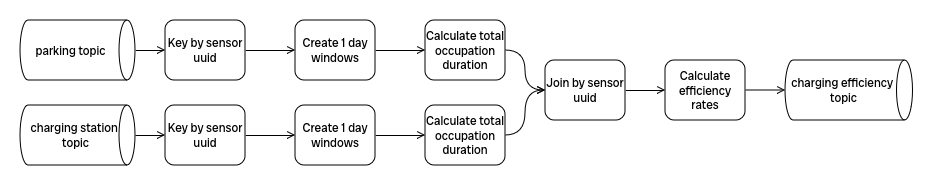
\includegraphics[width=0.9\textwidth]{./specifica_tecnica/charging_efficiency_flow.png}
	\captionof{figure}{Flusso di dati del \href{https://7last.github.io/docs/pb/documentazione-interna/glossario\#job}{\textit{job}\textsubscript{G}} \textit{Charging Efficiency}}
\end{center}
Le seguenti operazioni vengono eseguite indipendentemente per i dati provenienti dai \href{https://7last.github.io/docs/pb/documentazione-interna/glossario\#topic}{\textit{topic}\textsubscript{G}} relativi ai parcheggi e alle colonnine elettriche:
\begin{enumerate}
	\item lettura dei dati grezzi dai \href{https://7last.github.io/docs/pb/documentazione-interna/glossario\#topic}{\textit{topic}\textsubscript{G}} relativi ai parcheggi e alle colonnine elettriche, attraverso la classe \texttt{KafkaSource};
	\item assegnazione di un \textit{watermark} ai dati, come precedentemente descritto nel paragrafo \hyperref[watermark]{\underline{\textit{watermark}}};
	\item raggruppamento di dati utilizzando come chiave il \texttt{group\_name}, tramite la funzione \texttt{\mySkip{keyBy}} fornita da Flink;
	\item creazione di una finestra temporale di un giorno, utilizzando la funzione \texttt{window} di Flink;
	\item calcolo del tempo totale in cui le colonnine sono in uso e del tempo totale in cui i parcheggi sono occupati, utilizzando rispettivamente le classi
	      \\\texttt{ChargingStationTimeDifferenceWindowFunction} e \texttt{ParkingTimeDifferenceWindowFunction}.
\end{enumerate}
Successivamente, attraverso l'utilizzo dell'operatore \texttt{join} si uniscono i due \textit{stream} di dati, calcolando
attraverso la classe \texttt{ChargingEfficiencyJoinFunction} il valore dell'\textit{utilization rate} e dell'\textit{efficiency rate}.
Infine, i risultati vengono pubblicati nel \href{https://7last.github.io/docs/pb/documentazione-interna/glossario\#topic}{\textit{topic}\textsubscript{G}} dedicato all'efficienza delle colonnine elettriche.

\subsubsubsubsection{Architettura}
Analogamente a quanto svolto per il \href{https://7last.github.io/docs/pb/documentazione-interna/glossario\#job}{\textit{job}\textsubscript{G}} \href{https://7last.github.io/docs/pb/documentazione-interna/glossario\#heat-index}{\textit{Heat Index}\textsubscript{G}}, anche per il \href{https://7last.github.io/docs/pb/documentazione-interna/glossario\#job}{\textit{job}\textsubscript{G}} \textit{Charging Efficiency} è stata definita la
classe \texttt{ChargingEfficiencyJob}, la quale funge da punto di ingresso per l'esecuzione del \href{https://7last.github.io/docs/pb/documentazione-interna/glossario\#job}{\textit{job}\textsubscript{G}}. Essa definisce come sorgente di dati
i \href{https://7last.github.io/docs/pb/documentazione-interna/glossario\#topic}{\textit{topic}\textsubscript{G}} relativi all'occupazione dei parcheggi e delle colonnine elettriche, prepara l'esecuzione del \href{https://7last.github.io/docs/pb/documentazione-interna/glossario\#job}{\textit{job}\textsubscript{G}} e infine lo avvia
attraverso il metodo \texttt{execute}.\\

\begin{center}
	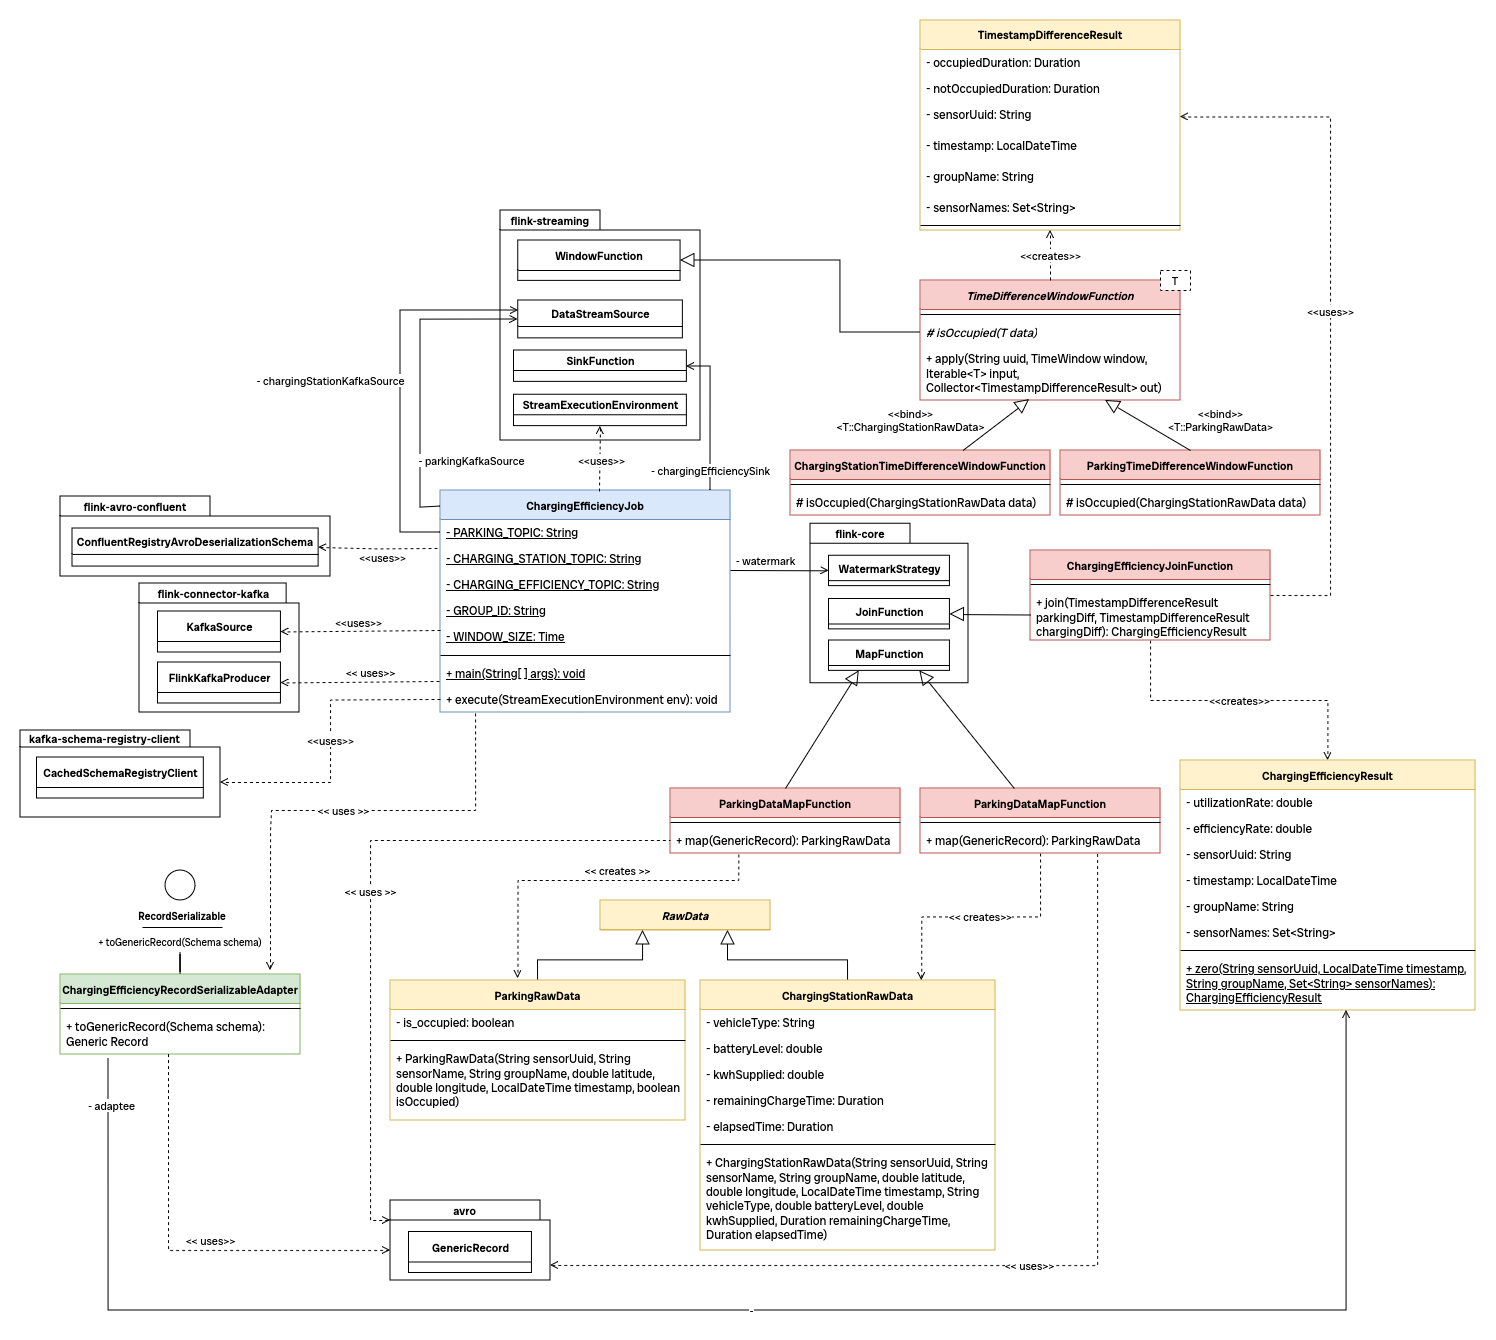
\includegraphics[width=1\textwidth]{./specifica_tecnica/charging_efficiency_job.png}
	\captionof{figure}{Architettura del \href{https://7last.github.io/docs/pb/documentazione-interna/glossario\#job}{\textit{job}\textsubscript{G}} \textit{Charging Efficiency}}
\end{center}

\subsubsubsubsubsection{\textit{Object adapter}}
La classe \texttt{ChargingEfficiencyResult} è stata adattata in un oggetto di tipo \texttt{GenericRecord} attraverso la classe \texttt{ChargingEfficiencyRecordSerializableAdapter},
analogamente a quanto descritto nella sezione \hyperref[object_adapter]{\underline{\textit{Object adapter}}}.

\subsubsubsubsubsection{\textit{Template method}}
Per poter ottenere il tempo totale in cui le colonnine e i parcheggi sono in uso in un certo periodo di tempo è necessario utilizzare una \texttt{WindowFunction},
funzione di Flink che si occupa di calcolare una determinata aggregazione in una finestra temporale. In questo caso, si occupa calcolare la somma delle differenze
tra due misurazioni consecutive in cui i kilowattora erogati dalle colonnine sono maggiori di 0 o i parcheggi sono occupati.\\
Risulta quindi evidente che le due funzioni di aggregazione sono molto simili tra loro, differendo solo per il campo utilizzato per determinare se la misurazione
è relativa ad un momento in cui le colonnine sono in uso o i parcheggi sono occupati. Per evitare di duplicare il codice, abbiamo deciso di utilizzare il \textit{pattern}
\textit{template method}, definendo una classe astratta \texttt{TimeDifferenceWindowFunction} che implementa l'interfaccia \texttt{WindowFunction}
e utilizza un \textit{generic type} \texttt{T extends RawData} per rappresentare il tipo di dato su cui effettuare l'aggregazione.
\texttt{TimeDifferenceWindowFunction} definisce un metodo astratto \texttt{isOccupied(T data)} che restituisce \texttt{true} se il dato passato come argomento è relativo ad una misurazione in cui
l'entità è in uso, \texttt{false} altrimenti. Inoltre, siccome implementa \texttt{WindowFunction}, deve ridefinire il metodo \texttt{apply}.
Riassumendo:
\begin{itemize}
	\item \texttt{isOccupied} è un metodo astratto e nel contesto del \textit{pattern} \textit{template method} è un metodo primitivo;
	\item \texttt{apply} è un metodo concreto e \texttt{final} e costituisce il \textit{template method};
	\item non sono presenti \textit{hook}, ovvero metodi che possono opzionalmente essere sovrascritti dalle sottoclassi, definiti con implementazione di \textit{default} nella \href{https://7last.github.io/docs/pb/documentazione-interna/glossario\#superclasse}{superclasse\textsubscript{G}}.
\end{itemize}

\subsubsubsubsubsection{Classi, interfacce metodi e attributi}
\begin{itemize}
	\item \textbf{Classe astratta RawData}: precedentemente descritta nella sezione relativa al \\\hyperref[abstract_class_raw_data]{\href{https://7last.github.io/docs/pb/documentazione-interna/glossario\#job}{\textit{\underline{job}}\textsubscript{G}}\underline{\textit{ \href{https://7last.github.io/docs/pb/documentazione-interna/glossario\#heat-index}{Heat Index\textsubscript{G}}}}};
	\item \textbf{Classe ParkingRawData}
	      \begin{itemize}
		      \item \textbf{Attributi}
		            \begin{itemize}
			            \item \texttt{is\_occupied} boolean [private]: valore che indica se il parcheggio è occupato o meno.
		            \end{itemize}
	      \end{itemize}
	\item \textbf{Classe ChargingStationRawData}
	      \begin{itemize}
		      \item \textbf{Attributi}
		            \begin{itemize}
			            \item \texttt{vehicleType} String [private]: tipo di veicolo che la colonnina ricarica;
			            \item \texttt{batteryLevel} double [private]: livello di batteria del veicolo collegato alla colonnina;
			            \item \texttt{kwhSupplied} double [private]: kilowattora che la colonnina sta erogando al momento della misurazione;
			            \item \texttt{remainingChargeTime} Duration [private]: tempo di ricarica rimanente;
			            \item \texttt{elapsedTime} Duration [private]: tempo di ricarica trascorso;
		            \end{itemize}
	      \end{itemize}
	\item \textbf{Classe ChargingEfficiencyJob}
	      \begin{itemize}
		      \item \textbf{Attributi}
		            \begin{itemize}
			            \item \texttt{PARKING\_TOPIC} str [private,final,static]: nome del \href{https://7last.github.io/docs/pb/documentazione-interna/glossario\#topic}{\textit{topic}\textsubscript{G}} relativo all'occupazione dei parcheggi;
			            \item \texttt{CHARGING\_STATION\_TOPIC} str [private,final,static]: nome del \href{https://7last.github.io/docs/pb/documentazione-interna/glossario\#topic}{\textit{topic}\textsubscript{G}} relativo all'utilizzo delle colonnine di ricarica;
			            \item \texttt{CHARGING\_EFFICIENCY\_TOPIC} str [private,final,static]: nome del \href{https://7last.github.io/docs/pb/documentazione-interna/glossario\#topic}{\textit{topic}\textsubscript{G}} relativo all'efficienza delle colonnine;
			            \item \texttt{GROUP\_ID} str [private,final,static]: identificativo del gruppo di consumatori;
			            \item \texttt{WINDOW\_SIZE} int [private,final,static]: dimensione della finestra temporale per cui calcolare le aggregazioni.
		            \end{itemize}
		      \item \textbf{Metodi}
		            \begin{itemize}
			            \item \texttt{main(String[] \mySkip{args})} [public,static]: metodo principale che si occupa di inizializzare l'ambiente di esecuzione, definire sorgente e \textit{sink} dei dati ed eseguire il \href{https://7last.github.io/docs/pb/documentazione-interna/glossario\#job}{\textit{job}\textsubscript{G}} vero e proprio;

			            \item \texttt{execute(StreamExecutionEnvironment \mySkip{env})} [public]: metodo che applica le trasformazioni a partire dai \textit{source} definiti nel metodo \textit{main}.
		            \end{itemize}
	      \end{itemize}
	\item \textbf{Classe astratta TimeDifferenceWindowFunction}
	      \begin{itemize}
		      \item \textbf{Metodi}
		            \begin{itemize}
			            \item \texttt{isOccupied(T data)} boolean [protected,abstract]: metodo che restituisce \texttt{true} se il dato passato come argomento è relativo ad una misurazione in cui l'entità è in uso, \texttt{false} altrimenti;
			            \item \texttt{apply(String uuid, TimeWindow window, Iterable<T> input,} \\\texttt{Collector<TimestampDifferenceResult> out)} void [public]: metodo
			                  che calcola il tempo totale in cui una data entità (colonnine o parcheggi) sono in uso in un certo periodo di tempo.
		            \end{itemize}
	      \end{itemize}
	\item \textbf{Classe ChargingStationTimeDifferenceWindowFunction}
	      \begin{itemize}
		      \item \textbf{Metodi}
		            \begin{itemize}
			            \item \texttt{isOccupied(ChargingStationRawData data)} boolean [protected]: metodo che restituisce \texttt{true} se il dato passato come argomento è relativo ad una misurazione in cui le colonnine sono in uso, \texttt{false} altrimenti.
		            \end{itemize}
		      \item \textbf{Note}
		            \begin{itemize}
			            \item \texttt{ChargingStationTimeDifferenceWindowFunction} estende la classe \\\texttt{TimeDifferenceWindowFunction} e implementa il metodo \texttt{isOccupied}.
		            \end{itemize}
	      \end{itemize}
	\item \textbf{Classe ParkingTimeDifferenceWindowFunction}
	      \begin{itemize}
		      \item \textbf{Metodi}
		            \begin{itemize}
			            \item \texttt{isOccupied(ParkingTimeDifferenceWindowFunction data)} boolean [protected]: metodo che restituisce \texttt{true} se il dato passato come argomento è relativo ad una misurazione in cui i
			                  parcheggi sono occupati, \texttt{false} altrimenti.
		            \end{itemize}
		      \item \textbf{Note}
		            \begin{itemize}
			            \item \texttt{ParkingTimeDifferenceWindowFunction} estende la classe \\\texttt{TimeDifferenceWindowFunction} e implementa il metodo \texttt{isOccupied}.
		            \end{itemize}
	      \end{itemize}
	\item \textbf{Classe TimestampDifferenceResult}
	      \begin{itemize}
		      \item \textbf{Attributi}
		            \begin{itemize}
			            \item \texttt{occupiedDuration} Duration [private]: durata in cui l'entità è in uso;
			            \item \texttt{notOccupiedDuration} Duration [private]: durata in cui l'entità non è in uso;
			            \item \texttt{sensorUuid} String [private]: identificativo univoco del \href{https://7last.github.io/docs/pb/documentazione-interna/glossario\#sensore}{sensore\textsubscript{G}};
			            \item \texttt{timestamp} LocalDateTime [private]: data e ora di inizio della finestra temporale in cui sono state calcolate le durate di occupazione e non occupazione;
			            \item \texttt{groupName} String [private]: nome del gruppo di sensori a cui appartiene il \href{https://7last.github.io/docs/pb/documentazione-interna/glossario\#sensore}{sensore\textsubscript{G}};
			            \item \texttt{\mySkip{sensorNames}} Set<String> [private]: insieme dei nomi dei sensori che hanno prodotto le misurazioni.
		            \end{itemize}
	      \end{itemize}
	\item \textbf{Classe ChargingEfficiencyJoinFunction}
	      \begin{itemize}
		      \item \texttt{join(TimestampDifferenceResult parkingDiff, \\TimestampDifferenceResult chargingDiff)}: calcola \textit{efficiency} e \textit{utilization rate} a partire da \texttt{TimestampDifferenceResult}
		            di parcheggi e colonnine.
	      \end{itemize}
	\item \textbf{Classe ChargingEfficiencyResult}

	      \begin{itemize}
		      \item \textbf{Attributi}:
		            \begin{itemize}
			            \item \texttt{utilizationRate} double [private]: tasso di utilizzo della colonnina di ricarica;
			            \item \texttt{efficiencyRate} double [private]: tasso di efficienza della colonnina di ricarica;
			            \item \texttt{sensorUuid} String [private]: identificativo univoco del \href{https://7last.github.io/docs/pb/documentazione-interna/glossario\#sensore}{sensore\textsubscript{G}};
			            \item \texttt{timestamp} LocalDateTime [private]: data e ora di inizio della finestra temporale in cui sono state calcolate le durate di occupazione e non occupazione;
			            \item \texttt{groupName} String [private]: nome del gruppo di sensori a cui appartiene il \href{https://7last.github.io/docs/pb/documentazione-interna/glossario\#sensore}{sensore\textsubscript{G}};
			            \item \texttt{\mySkip{sensorNames}} Set<String> [private]: insieme dei nomi dei sensori che hanno prodotto le misurazioni.
		            \end{itemize}
		      \item \textbf{Metodi}:
		            \begin{itemize}
			            \item \texttt{zero(String sensorUuid, LocalDateTime timestamp, String groupName,}\\
			                  \texttt{Set<String> sensorNames)} ChargingEfficiencyResult [public,static]: metodo che costruisce e ritorna un'istanza di ChargingEfficiencyResult
			                  con \\\texttt{utilizationRate} e \texttt{efficiencyRate} posti a 0.
		            \end{itemize}
	      \end{itemize}
	\item \textbf{Classe ParkingRawDataMapFunction}
	      \begin{itemize}
		      \item \textbf{Metodi}
		            \begin{itemize}
			            \item \texttt{map(GenericRecord record)} ParkingRawData [public]: metodo che converte un \texttt{GenericRecord} in un oggetto di tipo \texttt{ParkingRawData}.
		            \end{itemize}
	      \end{itemize}
	\item \textbf{Classe ChargingStationRawDataMapFunction}
	      \begin{itemize}
		      \item \textbf{Metodi}
		            \begin{itemize}
			            \item \texttt{map(GenericRecord record)} ChargingStationRawData [public]: metodo che converte un \texttt{GenericRecord} in un oggetto di tipo \texttt{ChargingStationRawData}.
		            \end{itemize}
	      \end{itemize}
	\item \textbf{Interfaccia RecordSerializable}: precedentemente descritta nella sezione relativa al \hyperref[record_serializable]{\href{https://7last.github.io/docs/pb/documentazione-interna/glossario\#job}{\textit{\underline{job}}\textsubscript{G}}\underline{\textit{ \href{https://7last.github.io/docs/pb/documentazione-interna/glossario\#heat-index}{Heat Index\textsubscript{G}}}}};
	\item \textbf{Classe ChargingEfficiencyRecordSerializableAdapter}
	      \begin{itemize}
		      \item \textbf{Attributi}
		            \begin{itemize}
			            \item \texttt{adaptee} ChargingEfficiencyResult [private, final]: oggetto da adattare.
		            \end{itemize}
		      \item \textbf{Metodi}
		            \begin{itemize}
			            \item \texttt{toGenericRecord()} GenericRecord [public]: metodo che restituisce un oggetto di tipo \texttt{GenericRecord} a partire da \texttt{adaptee}.
		            \end{itemize}
	      \end{itemize}
\end{itemize}

\subsection{ClickHouse}
\href{https://7last.github.io/docs/pb/documentazione-interna/glossario\#clickhouse}{ClickHouse\textsubscript{G}} viene utilizzato per memorizzare i dati grezzi provenienti dai sensori, i risultati delle elaborazioni effettuate da Apache Flink e i dati aggregati tramite
\href{https://7last.github.io/docs/pb/documentazione-interna/glossario\#materialized-view}{\textit{Materialized View}\textsubscript{G}}.\\

\subsubsection{Funzionalità utilizzate}
\subsubsubsection{\textit{Materialized View}}
Le \href{https://7last.github.io/docs/pb/documentazione-interna/glossario\#materialized-view}{\textit{Materialized View}\textsubscript{G}} in \href{https://7last.github.io/docs/pb/documentazione-interna/glossario\#clickhouse}{ClickHouse\textsubscript{G}} sono un meccanismo per memorizzare fisicamente i risultati di una \textit{query} specifica di selezione,
che viene periodicamente aggiornata in base ai dati sottostanti. Questo meccanismo consente di migliorare le prestazioni delle \textit{query} complesse
e di semplificare l'architettura del sistema, riducendo la necessità di eseguire \textit{query} costose e complesse ogni volta che si accede ai dati.

All'interno del progetto sono state utilizzate ai seguenti scopi:
\begin{itemize}
	\item \textbf{calcolo aggregazioni}: per calcolare la media aritmetica delle misurazioni per un certo periodo di tempo;
	\item \textbf{miglioramento prestazioni}: per rendere più efficienti le \textit{query} utilizzate più frequentemente per il popolamento di grafici e \href{https://7last.github.io/docs/pb/documentazione-interna/glossario\#dashboard}{dashboard\textsubscript{G}};
\end{itemize}

La documentazione è disponibile al seguente link:
\begin{center}
	\url{https://clickhouse.com/docs/en/guides/developer/cascading-materialized-views} [Ultima consultazione 2024-06-05]
\end{center}

\subsubsubsection{MergeTree}
MergeTree è uno dei principali motori di archiviazione di \href{https://7last.github.io/docs/pb/documentazione-interna/glossario\#clickhouse}{ClickHouse\textsubscript{G}}, progettato per gestire grandi volumi di dati e fornire elevate prestazioni di lettura e scrittura. È particolarmente adatto per applicazioni in cui i dati vengono aggiunti in modo incrementale e le \textit{query} vengono eseguite su intervalli di tempo specifici.
Le caratteristiche principali sono:
\begin{itemize}
	\item \textbf{partizionamento}, in cui i dati vengono partizionati in base a una colonna di data o di tempo, in modo che i dati più recenti siano memorizzati in partizioni separate e possano essere facilmente eliminati o archiviati;
	\item \textbf{ordine dei dati}, dove i dati vengono ordinati in base a una colonna di ordinamento, in modo che i dati siano memorizzati in modo sequenziale e possano essere letti in modo efficiente;
	\item \textbf{indice primario}, tramite il quale i dati vengono indicizzati in base a una colonna di chiave primaria, in modo che le \textit{query} di ricerca e di \textit{join} siano veloci ed efficienti;
	\item \textbf{\textit{merging} dei dati}, in questo modo i dati vengono uniti in modo incrementale in background, in modo che le \textit{query} di aggregazione e di analisi siano veloci ed efficienti;
	\item \textbf{compressione}, i dati vengono compressi in modo efficiente per ridurre lo spazio di archiviazione e migliorare le prestazioni di lettura e scrittura;
	\item \textbf{replica e distribuzione}, i dati possono essere replicati e distribuiti su più nodi per garantire l'affidabilità e la disponibilità del sistema.
\end{itemize}

La documentazione è disponibile al seguente link:
\begin{center}
	\url{https://clickhouse.com/docs/en/engines/table-engines/mergetree-family/mergetree} [Ultima consultazione 2024-06-05]
\end{center}

\subsubsection{Struttura}
Per ciascuna tipologia di dati o aggregazioni è stata definita una tabella all'interno del database \texttt{sensors}, mantenendo il nome esatto del \href{https://7last.github.io/docs/pb/documentazione-interna/glossario\#topic}{\textit{topic}\textsubscript{G}}
da cui provengono i dati.\\
Le tabelle di questo tipo vengono popolate da \href{https://7last.github.io/docs/pb/documentazione-interna/glossario\#redpanda}{Redpanda\textsubscript{G}} Connect, come precedentemente descritto nella \hyperref[redpanda_connect]{\underline{sezione apposita}}.
Per alcune tipologie di dati viene inoltre definita una \href{https://7last.github.io/docs/pb/documentazione-interna/glossario\#materialized-view}{\textit{Materialized View}\textsubscript{G}} che calcola aggregazioni sui dati grezzi,
in modo da rendere più efficienti le \textit{query} che necessitano di tali elaborazioni.
In particolare, viene calcolata la media aritmetica delle misurazioni per un certo periodo di tempo (differente a seconda del tipo di \href{https://7last.github.io/docs/pb/documentazione-interna/glossario\#sensore}{sensore\textsubscript{G}} e meglio descritto nelle sezioni seguenti),
dato frequentemente utilizzato per il popolamento di grafici e \href{https://7last.github.io/docs/pb/documentazione-interna/glossario\#dashboard}{\textit{dashboard}\textsubscript{G}} in \href{https://7last.github.io/docs/pb/documentazione-interna/glossario\#grafana}{Grafana\textsubscript{G}} e che dunque necessita di essere calcolato in modo efficiente.

\subsubsubsection{Misurazioni \textit{air quality}}
Di seguito viene rappresentata la tabella che contiene le misurazioni relative alla qualità dell'aria. Essa viene popolata da \href{https://7last.github.io/docs/pb/documentazione-interna/glossario\#redpanda}{Redpanda\textsubscript{G}} Connect ed utilizza il motore di \textit{storage}
MergeTree, il quale è ottimizzato per archiviare ed analizzare dati ordinati cronologicamente, in modalità \textit{append-only}; il suo
utilizzo è motivato dal fatto che tali misurazioni sono generalmente ordinate cronologicamente.

\begin{center}
	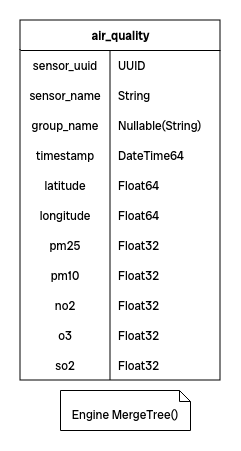
\includegraphics[width=0.25\textwidth]{./specifica_tecnica/air_quality_mv.png}
	\captionof{figure}{Tabella \texttt{air\_quality}}
\end{center}
\subsubsubsection{Misurazioni \textit{parking}}
Di seguito viene rappresentata la tabella che contiene le misurazioni relative all'occupazione dei parcheggi. Essa viene popolata da \href{https://7last.github.io/docs/pb/documentazione-interna/glossario\#redpanda}{Redpanda\textsubscript{G}} Connect ed utilizza il motore di \textit{storage}
MergeTree, il quale è ottimizzato per archiviare ed analizzare dati ordinati cronologicamente, in modalità \textit{append-only}; il suo
utilizzo è motivato dal fatto che tali misurazioni sono generalmente ordinate cronologicamente.
\begin{center}
	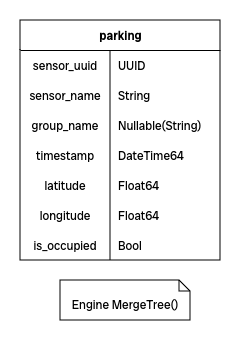
\includegraphics[width=0.25\textwidth]{./specifica_tecnica/parking_mv.png}
	\captionof{figure}{Tabella \texttt{parking}}
\end{center}
\subsubsubsection{Misurazioni \textit{recycling point}}
Di seguito viene rappresentata la tabella che contiene le misurazioni relative al riempimento delle isole ecologiche. Essa viene popolata da \href{https://7last.github.io/docs/pb/documentazione-interna/glossario\#redpanda}{Redpanda\textsubscript{G}} Connect ed utilizza il motore di \textit{storage}
MergeTree, il quale è ottimizzato per archiviare ed analizzare dati ordinati cronologicamente, in modalità \textit{append-only}; il suo
utilizzo è motivato dal fatto che tali misurazioni sono generalmente ordinate cronologicamente.
\begin{center}
	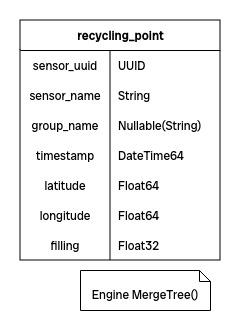
\includegraphics[width=0.25\textwidth]{./specifica_tecnica/recycling_point_mv.png}
	\captionof{figure}{Tabella \texttt{recycling\_point}}
\end{center}
\subsubsubsection{Misurazioni \textit{temperature}}
Di seguito viene rappresentata la configurazione per l'archiviazione delle misurazioni di temperatura. La tabella \texttt{temperature} utilizza il motore di \textit{storage}
MergeTree, il quale è ottimizzato per archiviare ed analizzare dati ordinati cronologicamente, in modalità \textit{append-only}; il suo
utilizzo è motivato dal fatto che tali misurazioni sono generalmente ordinate cronologicamente.
Tramite l'utilizzo delle \href{https://7last.github.io/docs/pb/documentazione-interna/glossario\#materialized-view}{\textit{Materialized View}\textsubscript{G}} \texttt{temperature\_5m\_mv}, \texttt{temperature\_weekly\_mv} e \texttt{temperature\_daily\_mv}
è possibile aggregare e trasferire i dati sulle tabelle \texttt{temperature\_5m}, \texttt{temperature\_weekly} e \texttt{temperature\_daily},
che contengono rispettivamente la media delle misurazioni per 5 minuti, giornaliere e settimanali.
\begin{center}
	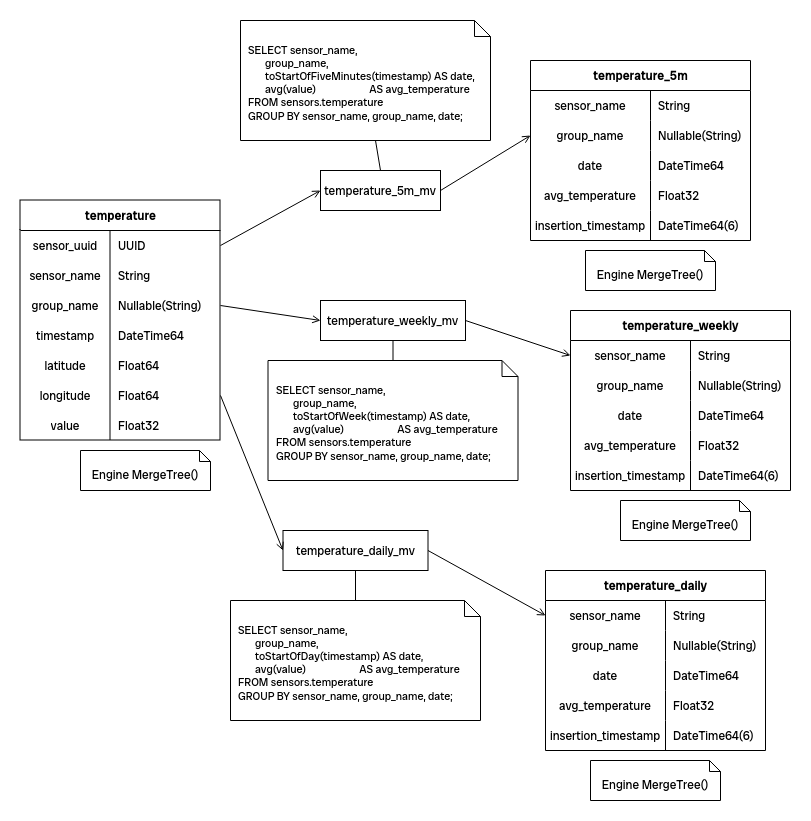
\includegraphics[width=0.9\textwidth]{./specifica_tecnica/temperature_mv.png}
	\captionof{figure}{Tabelle e \href{https://7last.github.io/docs/pb/documentazione-interna/glossario\#materialized-view}{\textit{materialized view}\textsubscript{G}} \texttt{temperature}}
\end{center}

\subsubsubsection{Misurazioni \textit{traffic}}
Di seguito viene rappresentata la configurazione per l'archiviazione delle misurazioni di temperatura. La tabella \texttt{traffic} utilizza il motore di \textit{storage}
MergeTree, il quale è ottimizzato per archiviare ed analizzare dati ordinati cronologicamente, in modalità \textit{append-only}; il suo
utilizzo è motivato dal fatto che tali misurazioni sono generalmente ordinate cronologicamente.
Tramite l'utilizzo della \href{https://7last.github.io/docs/pb/documentazione-interna/glossario\#materialized-view}{\textit{Materialized View}\textsubscript{G}} \texttt{traffic\_1h\_mv}
è possibile aggregare e trasferire i dati sulla tabella \texttt{traffic\_1h}, che contiene la media del numero di veicoli e velocità per ogni ora.
\begin{center}
	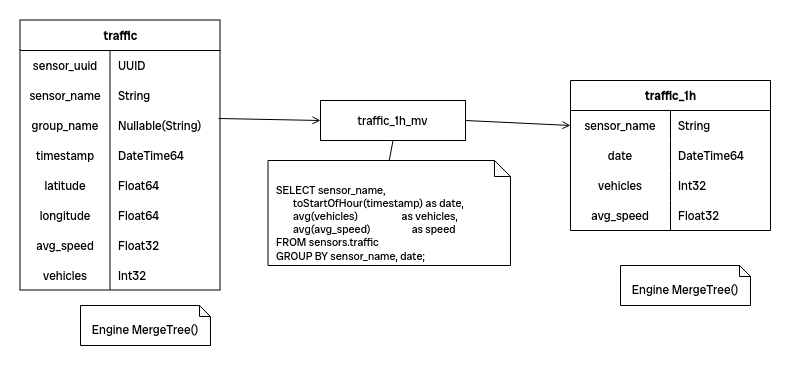
\includegraphics[width=0.9\textwidth]{./specifica_tecnica/traffic_mv.png}
	\captionof{figure}{Tabelle e \href{https://7last.github.io/docs/pb/documentazione-interna/glossario\#materialized-view}{\textit{materialized view}\textsubscript{G}} \texttt{traffic}}
\end{center}

\subsubsubsection{Misurazioni \textit{charging station}}
Di seguito viene rappresentata la configurazione per l'archiviazione delle misurazioni riguardanti l'occupazione delle colonnine di ricarica.
La tabella \texttt{charging\_station} utilizza il motore di \textit{storage} MergeTree, il quale è ottimizzato per archiviare ed analizzare dati ordinati cronologicamente,
in modalità \textit{append-only}; il suo utilizzo è motivato dal fatto che tali misurazioni sono generalmente ordinate cronologicamente.
Tramite l'utilizzo delle \href{https://7last.github.io/docs/pb/documentazione-interna/glossario\#materialized-view}{\textit{Materialized View}\textsubscript{G}} \texttt{charging\_station\_5m\_mv}, \texttt{charging\_station\_weekly\_mv} e \\\texttt{charging\_station\_daily\_mv}
è possibile aggregare e trasferire i dati sulle tabelle \\ \texttt{charging\_station\_5m}, \texttt{charging\_station\_weekly} e \texttt{charging\_station\_daily},
che contengono rispettivamente la media dei kilowattora erogati per 5 minuti, giornalmente e settimanalmente.
\begin{center}
	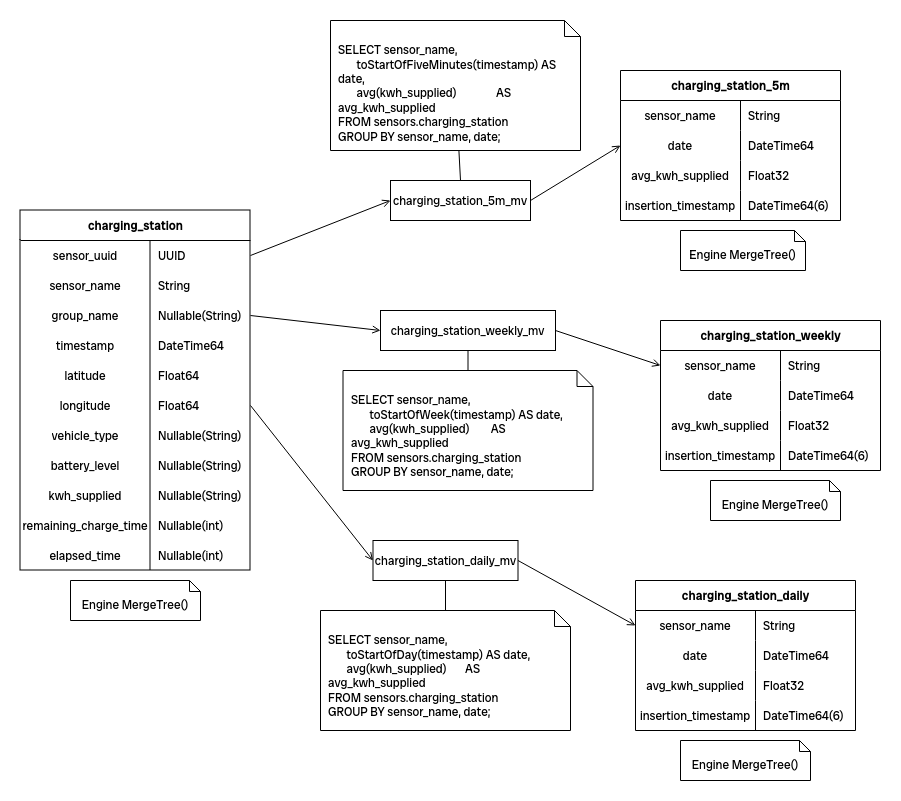
\includegraphics[width=0.9\textwidth]{./specifica_tecnica/charging_mv.png}
	\captionof{figure}{Tabelle e \href{https://7last.github.io/docs/pb/documentazione-interna/glossario\#materialized-view}{\textit{materialized view}\textsubscript{G}} \texttt{charging\_station}}
\end{center}

\subsubsubsection{Misurazioni \textit{precipitation}}
Di seguito viene rappresentata la configurazione per l'archiviazione delle misurazioni riguardanti le precipitazioni.
La tabella \texttt{precipitation} utilizza il motore di \textit{storage} MergeTree, il quale è ottimizzato per archiviare ed analizzare dati ordinati cronologicamente,
in modalità \textit{append-only}; il suo utilizzo è motivato dal fatto che tali misurazioni sono generalmente ordinate cronologicamente.
Tramite l'utilizzo delle \href{https://7last.github.io/docs/pb/documentazione-interna/glossario\#materialized-view}{\textit{Materialized View}\textsubscript{G}} \texttt{precipitation\_1h\_mv}, \texttt{precipitation\_daily\_mv}, \texttt{precipitation\_weekly\_mv} e \\\texttt{precipitation\_yearly\_mv} è possibile aggregare e trasferire i dati sulle tabelle \\\texttt{precipitation\_1h}, \texttt{precipitation\_daily}, \texttt{precipitation\_weekly} e \texttt{precipitation\_yearly}
che contengono la media dei millimetri di acqua caduti rispettivamente per ogni ora, giorno, settimana e anno.
\begin{center}
	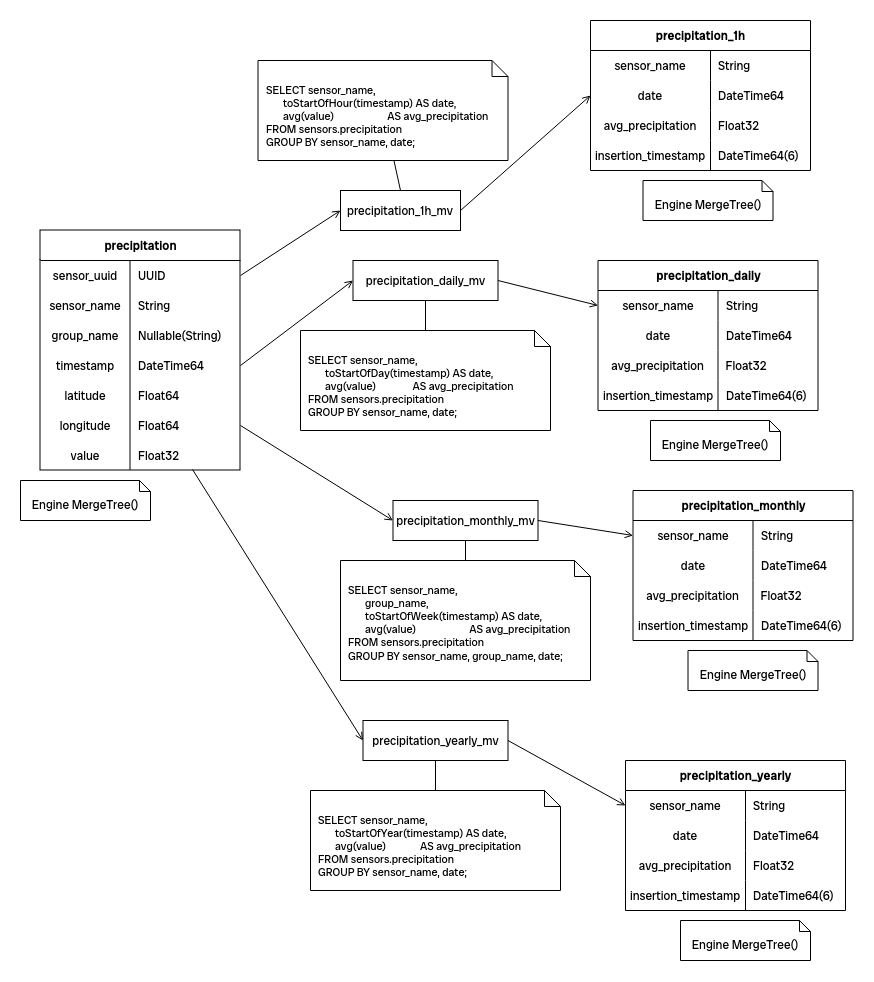
\includegraphics[width=0.8\textwidth]{./specifica_tecnica/precipitation_mv.png}
	\captionof{figure}{Tabelle e \href{https://7last.github.io/docs/pb/documentazione-interna/glossario\#materialized-view}{\textit{materialized view}\textsubscript{G}} \texttt{precipitation}}
\end{center}

\subsubsubsection{Misurazioni \textit{river level}}
Di seguito viene rappresentata la configurazione per l'archiviazione delle misurazioni riguardanti il livello dei fiumi.
La tabella \texttt{river\_level} utilizza il motore di \textit{storage} MergeTree, il quale è ottimizzato per archiviare ed analizzare dati ordinati cronologicamente,
in modalità \textit{append-only}; il suo utilizzo è motivato dal fatto che tali misurazioni sono generalmente ordinate cronologicamente.
Tramite l'utilizzo delle \href{https://7last.github.io/docs/pb/documentazione-interna/glossario\#materialized-view}{\textit{Materialized View}\textsubscript{G}} \texttt{river\_level\_1h\_mv}, \texttt{river\_level\_daily\_mv}, \texttt{river\_level\_weekly\_mv} e \texttt{river\_level\_yearly\_mv}
è possibile aggregare e trasferire i dati sulle tabelle \texttt{river\_level\_1h},\texttt{river\_level\_daily},\\ \texttt{river\_level\_weekly} e \texttt{river\_level\_yearly}
che contengono rispettivamente la media oraria, giornaliera, mensile e annuale del livello dei fiumi (misurato in metri).

\begin{center}
	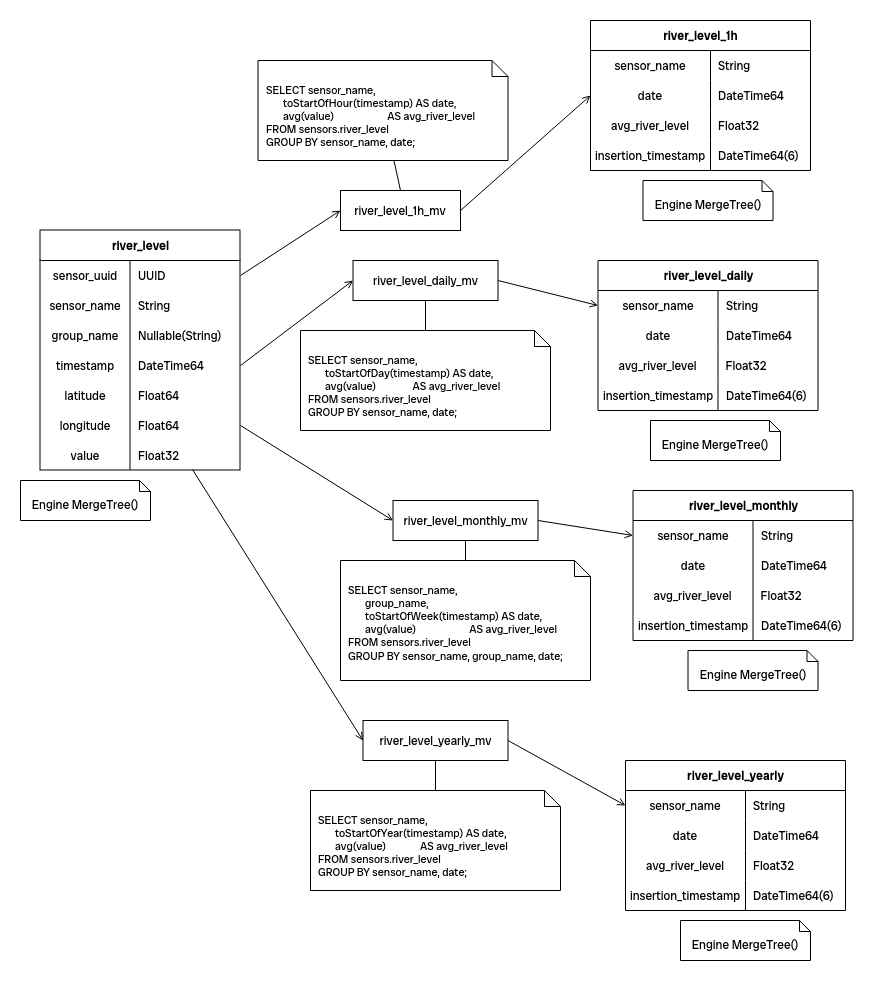
\includegraphics[width=0.8\textwidth]{./specifica_tecnica/river_mv.png}
	\captionof{figure}{Tabelle e \href{https://7last.github.io/docs/pb/documentazione-interna/glossario\#materialized-view}{\textit{materialized view}\textsubscript{G}} \texttt{river\_level}}
\end{center}

\subsubsubsection{Misurazioni \textit{humidity}}
Di seguito viene rappresentata la configurazione per l'archiviazione delle misurazioni di umidità. La tabella \texttt{humidity} utilizza il motore di \textit{storage}
MergeTree, il quale è ottimizzato per archiviare ed analizzare dati ordinati cronologicamente, in modalità \textit{append-only}; il suo
utilizzo è motivato dal fatto che tali misurazioni sono generalmente ordinate cronologicamente.
Tramite l'utilizzo delle \href{https://7last.github.io/docs/pb/documentazione-interna/glossario\#materialized-view}{\textit{Materialized View}\textsubscript{G}} \texttt{humidity\_5m\_mv}, \texttt{humidity\_weekly\_mv} e \texttt{humidity\_daily\_mv}
è possibile aggregare e trasferire i dati sulle tabelle \texttt{humidity\_5m}, \texttt{humidity\_weekly} e \texttt{humidity\_daily},
che contengono rispettivamente la media delle misurazioni di umidità relativa per 5 minuti, giornaliere e settimanali.
\begin{center}
	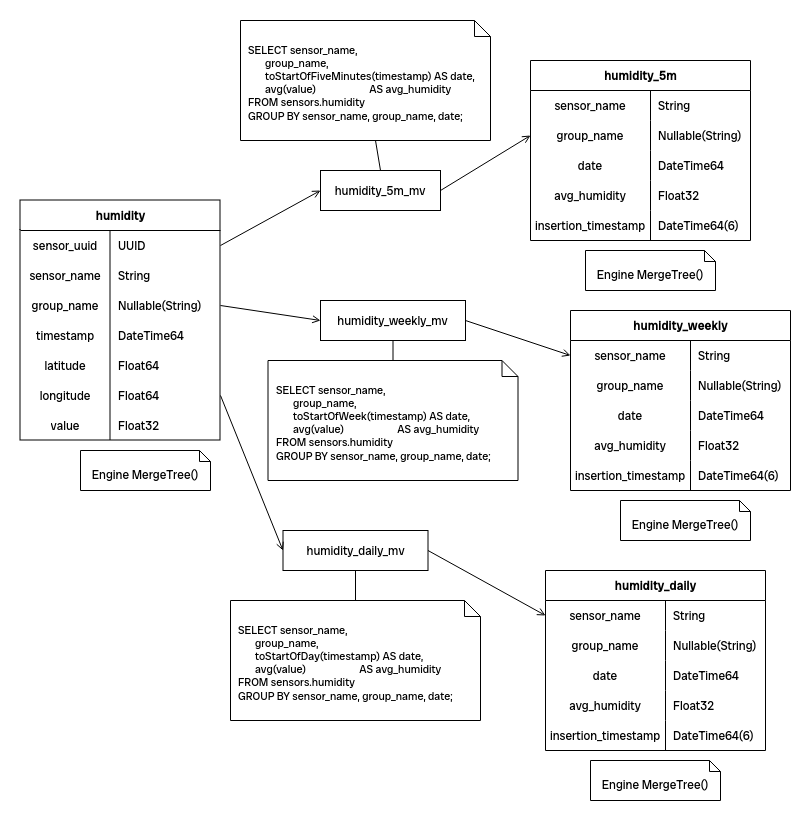
\includegraphics[width=0.8\textwidth]{./specifica_tecnica/humidity_mv.png}
	\captionof{figure}{Tabelle e \href{https://7last.github.io/docs/pb/documentazione-interna/glossario\#materialized-view}{\textit{materialized view}\textsubscript{G}} \texttt{humidity}}
\end{center}

\subsubsubsection{Misurazioni \textit{heat index}}
Di seguito viene rappresentata la configurazione per l'archiviazione delle misurazioni dello \textit{heat\_index}. La tabella \texttt{humidity} utilizza il motore di \textit{storage}
MergeTree, il quale è ottimizzato per archiviare ed analizzare dati ordinati cronologicamente, in modalità \textit{append-only}; il suo
utilizzo è motivato dal fatto che tali misurazioni sono generalmente ordinate cronologicamente.
Tramite l'utilizzo della \href{https://7last.github.io/docs/pb/documentazione-interna/glossario\#materialized-view}{\textit{Materialized View}\textsubscript{G}} \texttt{heat\_index\_daily\_mv} è possibile aggregare e trasferire i dati sulla tabella \texttt{heat\_index\_daily}
che contiene la media giornaliera delle misurazioni.

\begin{center}
	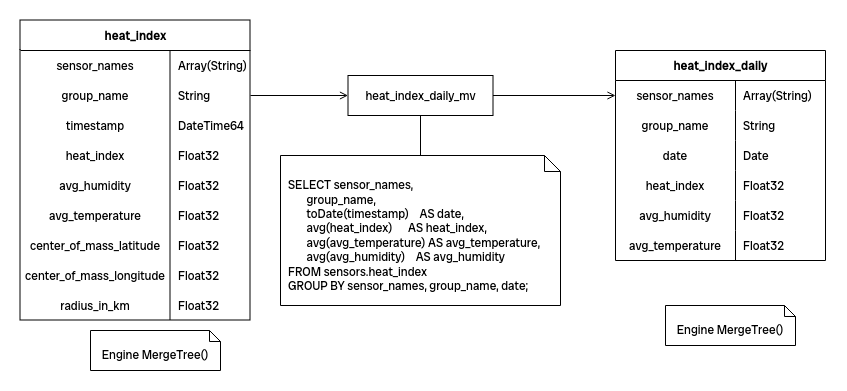
\includegraphics[width=0.9\textwidth]{./specifica_tecnica/heat_index_mv.png}
	\captionof{figure}{Tabelle e \href{https://7last.github.io/docs/pb/documentazione-interna/glossario\#materialized-view}{\textit{materialized view}\textsubscript{G}} \texttt{heat\_index}}
\end{center}

\subsubsubsection{Misurazioni \textit{charging efficiency}}
Di seguito viene rappresentata la tabella che contiene le misurazioni relative all'efficienza delle colonnine elettriche. Essa viene popolata da \href{https://7last.github.io/docs/pb/documentazione-interna/glossario\#redpanda}{Redpanda\textsubscript{G}} Connect ed utilizza il motore di \textit{storage}
MergeTree, il quale è ottimizzato per archiviare ed analizzare dati ordinati cronologicamente, in modalità \textit{append-only}; il suo
utilizzo è motivato dal fatto che tali misurazioni sono generalmente ordinate cronologicamente.

\begin{center}
	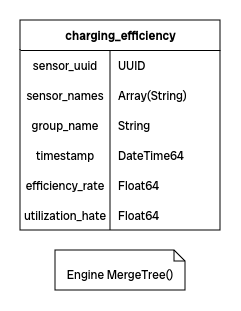
\includegraphics[width=0.35\textwidth]{./specifica_tecnica/charging_efficiency_mv.png}
	\captionof{figure}{Tabella \texttt{charging\_efficiency}}
\end{center}
\subsubsubsection{Tabella sensors}
In diversi scenari all'interno di \href{https://7last.github.io/docs/pb/documentazione-interna/glossario\#grafana}{Grafana\textsubscript{G}} è necessario poter ottenere i dati di tutti i sensori, indipendentemente dalla loro tipologia, per mostrarli ad esempio in una mappa
complessiva o in una tabella contenente la data di ricezione dell'ultimo messaggio da parte di un determinato dispositivo o ancora per la costruzione dei filtri su tipo e nome di ciascun \href{https://7last.github.io/docs/pb/documentazione-interna/glossario\#sensore}{sensore\textsubscript{G}}.
Al fine di rendere maggiormente efficiente queste operazioni abbiamo realizzato una tabella \texttt{sensors} popolata attraverso delle \href{https://7last.github.io/docs/pb/documentazione-interna/glossario\#materialized-view}{\textit{Materialized View}\textsubscript{G}},
che si occupano di trasferire i dati a partire dalle tabelle dei dati grezzi (come \texttt{temperature}, \texttt{humidity}...).
All'interno del commento contenuto nel diagramma seguente è presente un esempio generico di \textit{query} utilizzata per la definizione delle \href{https://7last.github.io/docs/pb/documentazione-interna/glossario\#materialized-view}{\textit{Materialized View}\textsubscript{G}}; al posto del \textit{placeholder}
\texttt{{type}} è sufficiente sostituire il nome di ciascuna tabella di dati grezzi (\texttt{temperature}, \texttt{humidity}...).
I campi di quest'ultime sono omessi per semplicità del diagramma e sono stati precedentemente illustrati nella sezione dedicata alle misurazioni di ciascuna tipologia.

\begin{center}
	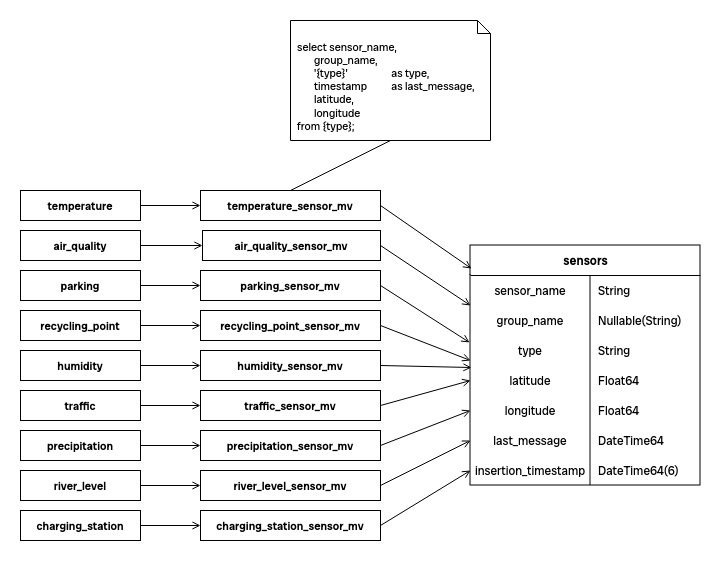
\includegraphics[width=0.9\textwidth]{./specifica_tecnica/sensors_mv.png}
	\captionof{figure}{Tabelle e \href{https://7last.github.io/docs/pb/documentazione-interna/glossario\#materialized-view}{\textit{materialized view}\textsubscript{G}} \texttt{sensors}}
\end{center}

\pagebreak
\subsection{Grafana}
\href{https://7last.github.io/docs/pb/documentazione-interna/glossario\#grafana}{Grafana\textsubscript{G}} è uno strumento di analisi e monitoraggio che permette di visualizzare dati provenienti da una varietà di fonti. È sviluppato principalmente in Go e Typescript e si è diffuso notevolmente
in quanto offre funzionalità per la creazione di \href{https://7last.github.io/docs/pb/documentazione-interna/glossario\#dashboard}{\textit{dashboard}\textsubscript{G}} personalizzabili e intuitive.
\subsubsection{Dashboard}
Sono state realizzate tre \href{https://7last.github.io/docs/pb/documentazione-interna/glossario\#dashboard}{\textit{dashboard}\textsubscript{G}} distinte, ciascuna per adempiere a uno specifico compito:
\begin{itemize}
	\item \textbf{\textit{Raw data}}: mostra i dati grezzi provenienti dai sensori in delle tabelle filtrabili. Inoltre contiene dei pannelli che consentono
	      di visualizzare informazioni generali sui sensori, come una mappa con la loro posizione e una tabella con l'ultimo messaggio ricevuto da ciascuno di essi.
	\item \textbf{\textit{Urban data}}: mostra i dati aggregati relativi a traffico, isole ecologiche, parcheggi e colonnine di ricarica. In particolare, sono presenti
	      grafici che mostrano l'andamento temporale delle misurazioni e delle aggregazioni calcolate.
	\item \textbf{\textit{Environmental data}}: mostra i dati aggregati relativi a qualità dell'aria, temperatura, umidità, precipitazioni, e livello dei fiumi.
	      Anche in questo caso sono presenti grafici che mostrano l'andamento temporale delle misurazioni e delle aggregazioni calcolate.
\end{itemize}
La suddivisione è stata progettata in questo modo in quanto, oltre al fatto che la natura dei dati sia molto differente, le varie \href{https://7last.github.io/docs/pb/documentazione-interna/glossario\#dashboard}{\textit{dashboard}\textsubscript{G}} potrebbero venire utilizzate dagli utenti con esigenze diverse:
i dati ambientali possono essere adoperati al fine di prevenire situazioni di emergenza correlate a condizioni climatiche avverse, mentre quelli urbanistici possono essere utilizzati con fini economici
o per migliorare i servizi offerti ai cittadini.

\subsubsection{ClickHouse datasource plugin}
Il plugin \href{https://7last.github.io/docs/pb/documentazione-interna/glossario\#clickhouse}{ClickHouse\textsubscript{G}} per \href{https://7last.github.io/docs/pb/documentazione-interna/glossario\#grafana}{Grafana\textsubscript{G}} è un'implementazione che consente di utilizzare \href{https://7last.github.io/docs/pb/documentazione-interna/glossario\#clickhouse}{ClickHouse\textsubscript{G}} come fonte di dati per \href{https://7last.github.io/docs/pb/documentazione-interna/glossario\#grafana}{Grafana\textsubscript{G}}. Questo plugin facilita la connessione e l'interrogazione dei dati archiviati in \href{https://7last.github.io/docs/pb/documentazione-interna/glossario\#clickhouse}{ClickHouse\textsubscript{G}} direttamente da \href{https://7last.github.io/docs/pb/documentazione-interna/glossario\#grafana}{Grafana\textsubscript{G}}.
La documentazione è disponibile al seguente link:
\begin{center}
	\url{https://grafana.com/grafana/plugins/grafana-clickhouse-datasource/} [Ultima consultazione 2024-06-05]
\end{center}
La configurazione di tale \textit{datasource} è contenuta nella cartella \\
\href{https://7last.github.io/docs/pb/documentazione-interna/glossario\#grafana}{\texttt{grafana}\textsubscript{G}}\texttt{/provisioning/datasources/default.\href{https://7last.github.io/docs/pb/documentazione-interna/glossario\#yet-another-markup-language}{yaml\textsubscript{G}}} della repository del progetto.

\subsubsection{Variabili Grafana}
Al fine di rendere le \href{https://7last.github.io/docs/pb/documentazione-interna/glossario\#dashboard}{\textit{dashboard}\textsubscript{G}} più flessibili e personalizzabili, sono state utilizzate le variabili di \href{https://7last.github.io/docs/pb/documentazione-interna/glossario\#grafana}{Grafana\textsubscript{G}}. Esse consentono di definire parametri dinamici che possono essere utilizzati per filtrare, raggruppare o personalizzare i dati visualizzati nei pannelli delle \href{https://7last.github.io/docs/pb/documentazione-interna/glossario\#dashboard}{dashboard\textsubscript{G}}.
La documentazione è disponibile al seguente link:
\begin{center}
	\url{https://grafana.com/docs/grafana/latest/dashboards/variables/} [Ultima consultazione 2024-06-05]
\end{center}
\subsubsubsection{Variabili nella \textit{dashboard} \textit{Raw data}}
\begin{itemize}
	\item \texttt{sensor\_type}: permette di filtrare i dati visualizzati in base al tipo di \href{https://7last.github.io/docs/pb/documentazione-interna/glossario\#sensore}{sensore\textsubscript{G}};
	\item \texttt{sensor\_name}: dipendente dalla variabile \texttt{sensor\_type} e permette di filtrare i dati visualizzati in base al nome del \href{https://7last.github.io/docs/pb/documentazione-interna/glossario\#sensore}{sensore\textsubscript{G}};
\end{itemize}

\subsubsubsection{Variabili nella \textit{dashboard} \textit{Urban data}}
\begin{itemize}
	\item \texttt{group\_name\_charging}: permette di filtrare i dati visualizzati in base al \texttt{group\_name} di colonnine di ricarica;
	\item \texttt{group\_name\_parking}: permette di filtrare i dati visualizzati in base al \texttt{group\_name} di parcheggi;
	\item \texttt{sensor\_name\_recycling\_point}: permette di filtrare i dati visualizzati in base al nome del \href{https://7last.github.io/docs/pb/documentazione-interna/glossario\#sensore}{sensore\textsubscript{G}} di isole ecologiche;
	\item \texttt{sensor\_name\_traffic}: permette di filtrare i dati visualizzati in base al nome del \href{https://7last.github.io/docs/pb/documentazione-interna/glossario\#sensore}{sensore\textsubscript{G}} di traffico;
\end{itemize}
\subsubsubsection{Variabili nella \textit{dashboard} \textit{Environmental data}}
\begin{itemize}
	\item \texttt{group\_name\_temperature}: permette di filtrare i dati visualizzati in base al \texttt{group\_name} di sensori di temperatura;
	\item \texttt{sensor\_name\_humidity}: permette di filtrare i dati visualizzati in base al \texttt{group\_name} di sensori di umidità;
	\item \texttt{sensor\_name\_precipitation}: permette di filtrare i dati visualizzati in base al \texttt{group\_name} di sensori di precipitazioni;
	\item \texttt{sensor\_name\_river\_level}: permette di filtrare i dati visualizzati in base al \texttt{group\_name} di sensori di livello dei fiumi;
	\item \texttt{sensor\_name\_air\_quality}: permette di filtrare i dati visualizzati in base al \texttt{group\_name} di sensori di qualità dell'aria;
\end{itemize}

\subsubsection{Grafana Alerts}
Gli \textit{alert} di \href{https://7last.github.io/docs/pb/documentazione-interna/glossario\#grafana}{Grafana\textsubscript{G}} sono una funzionalità che permettono di definire, configurare e gestire avvisi basati su condizioni specifiche rilevate nei dati monitorati. Questi avvisi consentono agli utenti di essere informati tempestivamente su eventuali problemi o cambiamenti critici nei loro sistemi, applicazioni o infrastrutture.\\
La documentazione è disponibile al seguente link:
\begin{center}
	\url{https://grafana.com/docs/grafana/latest/alerting/} [Ultima consultazione 2024-06-05]
\end{center}

\subsubsubsection{Configurazione delle regole di alert}
Definiscono le condizioni che devono essere soddisfatte per attivare un alert. Gli eventi che generano un alert sono:
\begin{itemize}
	\item temperatura maggiore di 40°C per più di 30 minuti;
	\item isola ecologica piena al 100\% per più di 24 ore;
	\item superamento dell'indice 3 dell'\href{https://7last.github.io/docs/pb/documentazione-interna/glossario\#european-air-quality-index}{EAQI\textsubscript{G}} (indice di qualità dell'aria);
	\item livello di precipitazioni superiore a 10 mm in 1 ora.
\end{itemize}
Gli alert possono possedere tre diversi tipi di stati:
\begin{itemize}
	\item \textbf{\textit{normal}}, indica che l'alert non è attivo perché le condizioni definite per l'attivazione dell'avviso non sono soddisfatte;
	\item \textbf{\textit{pending}}, indica che le metriche monitorate stanno iniziando a deviare dalle condizioni normali ma non hanno ancora soddisfatto completamente le condizioni per attivare l'alert;
	\item \textbf{\textit{firing}}, significa che le condizioni definite per l'avviso sono state soddisfatte e l'alert è attivo.
\end{itemize}
\subsubsubsection{Configurazione canale di notifica}
Per configurare un canale di notifica è necessario:
\begin{enumerate}
	\item nel menù di sinistra, cliccare sull'icona "Alerting";
	\item selezionare la voce "Notification channels";
	\item cliccare sul pulsante "Add channel" per aggiungere un nuovo canale di notifica;
	\item selezionare il tipo di canale di notifica desiderato tra quelli disponibili;
	\item configurare le impostazioni del canale di notifica in base alle proprie esigenze;
	\item cliccare sul pulsante "Save" per salvare le impostazioni del canale di notifica.
\end{enumerate}

\subsubsection{Altri plugin}
\subsubsubsection{Orchestra Cities Map plugin}
Progettato per facilitare la visualizzazione e l'analisi dei dati geospaziali all'interno di piattaforme di pianificazione urbana e sviluppo territoriale.\\
Le principali funzionalità offerte da questo plugin sono:
\begin{itemize}
	\item \textbf{visualizzazione dei dati geospaziali}: consente agli utenti di visualizzare dati geografici, come mappe, strati di dati \mySkip{GIS} (\textit{Geographic Information System}), punti di interesse e altre informazioni territoriali;
	\item \textbf{interfaccia interattiva}: offre un'interfaccia utente intuitiva e interattiva che consente agli utenti di esplorare e interagire con i dati geospaziali in modo dinamico;
	\item \textbf{personalizzazione}: offre opzioni di personalizzazione per adattarsi alle esigenze specifiche dell'utente o dell'applicazione;
	\item \textbf{analisi dei dati}: oltre alla semplice visualizzazione dei dati geospaziali, il plugin può anche supportare funzionalità avanzate di analisi dei dati, come l'identificazione di cluster, la creazione di heatmap e l'esecuzione di analisi spaziali per identificare tendenze o pattern significativi nei dati territoriali;
	\item \textbf{integrazione}: è progettato per integrarsi facilmente con altre componenti dell'ecosistema Orchestra Cities e con altre piattaforme software di pianificazione urbana e sviluppo territoriale.
\end{itemize}

La documentazione è disponibile al seguente link:
\begin{center}
	\url{https://grafana.com/grafana/plugins/orchestracities-map-panel/?tab=installation} [Ultima consultazione 2024-06-05]
\end{center}

